\documentclass[final]{beamer}
\usepackage{grffile}
\mode<presentation>{\usetheme{DMcDp}}
\usepackage[english]{babel}
\usepackage[latin1]{inputenc}
\usepackage{amsmath,amsthm, amssymb, latexsym}
\usepackage{pifont}
\usepackage{array}
\usepackage[orientation=landscape,size=custom,width=121.92,height=91.44,scale=1.5,debug]{beamerposter}
% change list indention level
% \setdefaultleftmargin{3em}{}{}{}{}{}

%\usepackage{snapshot} % will write a .dep file with all dependencies, allows for easy bundling

\usepackage{array,booktabs,tabularx}
\newcolumntype{Z}{>{\centering\arraybackslash}X} % centered tabularx columns
\newcommand{\given}{\mbox{ }\vert\mbox{ }}
\bibliographystyle{jasa}
\newcommand{\F}{\mathcal{F}}
\newcommand{\E}{\mathbb{E}}
\renewcommand{\P}{\mathbb{P}}
\newcommand{\R}{\mathbb{R}}
\newcommand{\X}{\mathcal{X}}
\newcommand{\B}{\mathcal{B}}
\newcommand{\V}{\mathbb{V}}
\newcommand{\Y}{\mathcal{Y}}
\newcommand{\bsp}{\boldsymbol{\phi}}
\DeclareMathOperator*{\argmin}{argmin} % thanks, wikipedia!
\newcommand{\TV}[1]{\left|\left| #1 \right|\right|_{TV}}
\newcommand{\joint}{\P_{1\otimes a}}

\newtheorem{propo}{Proposition}
\newenvironment{prop}{\begin{propo}}{\end{propo}} 

%\newcolumntype{Va}[1]{>{\centering\arraybackslash} m{.2\linewidth} }
%\newcolumntype{Vb}[1]{>{\centering\arraybackslash} m{.4\linewidth} }

\def\defgraphUnit#1#2#3#4{%
% {mark}{HEIGHT}{WIDTH}{mark}{code}
\setbox\csname dhgraph#1\endcsname{\vbox to #2{\hsize=#3\vss\hbox to #3{\hss#4\hss}\vss}}
}


\listfiles

%%%%%%%%%%%%%%%%%%%%%%%%%%%%%%%%%%%%%%%%%%%%%%%%%%%%%%%%%%%%%%%%%%%%%%%%%%%%%%%%%%%%%%

\title{\huge Efficient Estimators for Sequential and
Resolution-Limited Inverse Problems
}
%\author{Darren Homrighausen}
%\institute[CMU Statistics]{Department of Statistics, Carnegie Mellon University}
\author[Homrighausen,Genovese]{Darren Homrighausen \and Christopher R. Genovese}
\institute[CMU Statistics]{Department of Statistics, Carnegie Mellon University}
\date[]{}

%%%%%%%%%%%%%%%%%%%%%%%%%%%%%%%%%%%%%%%%%%%%%%%%%%%%%%%%%%%%%%%%%%%%%%%%%%%%%%%%%%%%%%
\newlength{\columnheight}
\setlength{\columnheight}{77cm}

%%%%%%%%%%%%%%%%%%%%%%%%%%%%%%%%%%%%%%%%%%%%%%%%%%%%%%%%%%%%%%%%%%%%%%%%%%%%%%%%%%%%%%
\begin{document}
\begin{frame}
  \begin{columns}

    \begin{column}{.32\textwidth}
      \begin{beamercolorbox}[center,wd=\textwidth]{postercolumn}
        \begin{minipage}[T]{.95\textwidth} 
          \parbox[t][\columnheight]{\textwidth}{
            % 
            \vfill
            % 
            \begin{block}{Sequential Inverse Problem: Notation}
              \begin{table}
\centering
\begin{tabular}{ccc}
& \includegraphics[width=2.6in,trim=100 225 0 235,clip]{./figures/inverseProblemEx2a.eps} 
& \includegraphics[width=2.6in,trim=100 225 0 235,clip]{./figures/inverseProblemEx3a.eps} \\
  \includegraphics[width=2.6in,trim=100 225 0 235,clip]{./figures/inverseProblemEx1.eps}
& \includegraphics[width=2.6in,trim=100 225 0 235,clip]{./figures/inverseProblemEx2b.eps} 
& \includegraphics[width=2.6in,trim=100 225 0 235,clip]{./figures/inverseProblemEx3b.eps} \\
& \includegraphics[width=2.6in,trim=100 225 0 235,clip]{./figures/inverseProblemEx2c.eps} 
& \includegraphics[width=2.6in,trim=100 225 0 235,clip]{./figures/inverseProblemEx3c.eps} \\
$\theta$ & $K_i\theta$ & $Y_i = K_i\theta + \epsilon Z$ 
\end{tabular}
\end{table}
            \end{block}
            \begin{block}{Two Data Analysis Examples: }
              \begin{table}
                \centering
                \begin{tabular}{c c c}
                  \begin{minipage}[r][1.5in][c]{3cm}
                  \end{minipage} &
                  \begin{minipage}[c][1.5in][c]{6in}
                  \textcolor{green!50!black}{Satellite Imaging}
                  \end{minipage} &
                  \begin{minipage}[c][1.5in][c]{6in}
                  \textcolor{green!50!black}{Observational Astronomy}
                  \end{minipage} 
                  \\
                  \begin{minipage}[r][2.5in][c]{3cm}
                  $\theta$
                  \end{minipage} &
                  \begin{minipage}[c][2.5in][c]{6in}
                    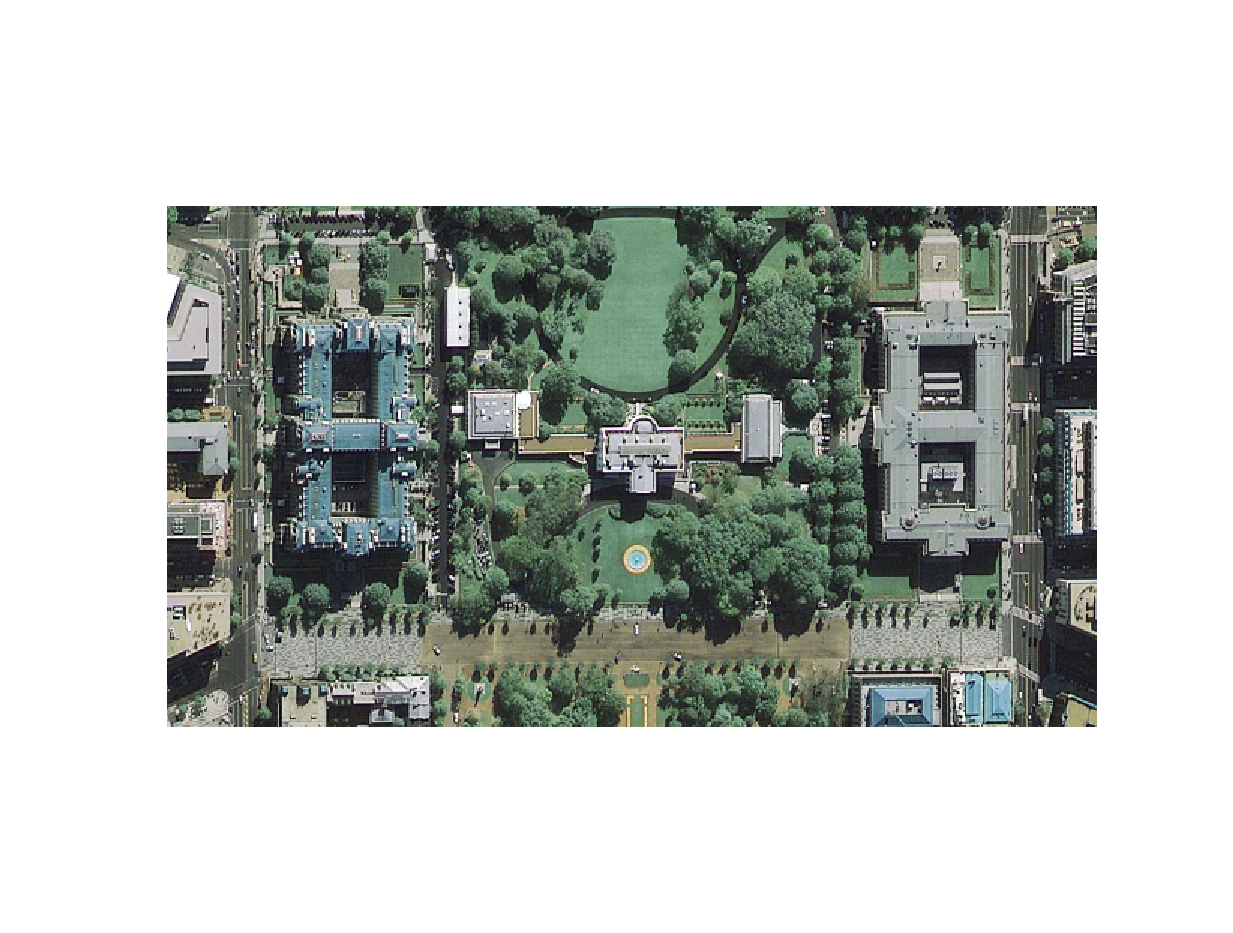
\includegraphics[width=5in,trim=80 130 80 90,clip]{./figures/satelliteColor.eps}
                  \end{minipage} &
                  \begin{minipage}[c][2.5in][c]{6in}
                  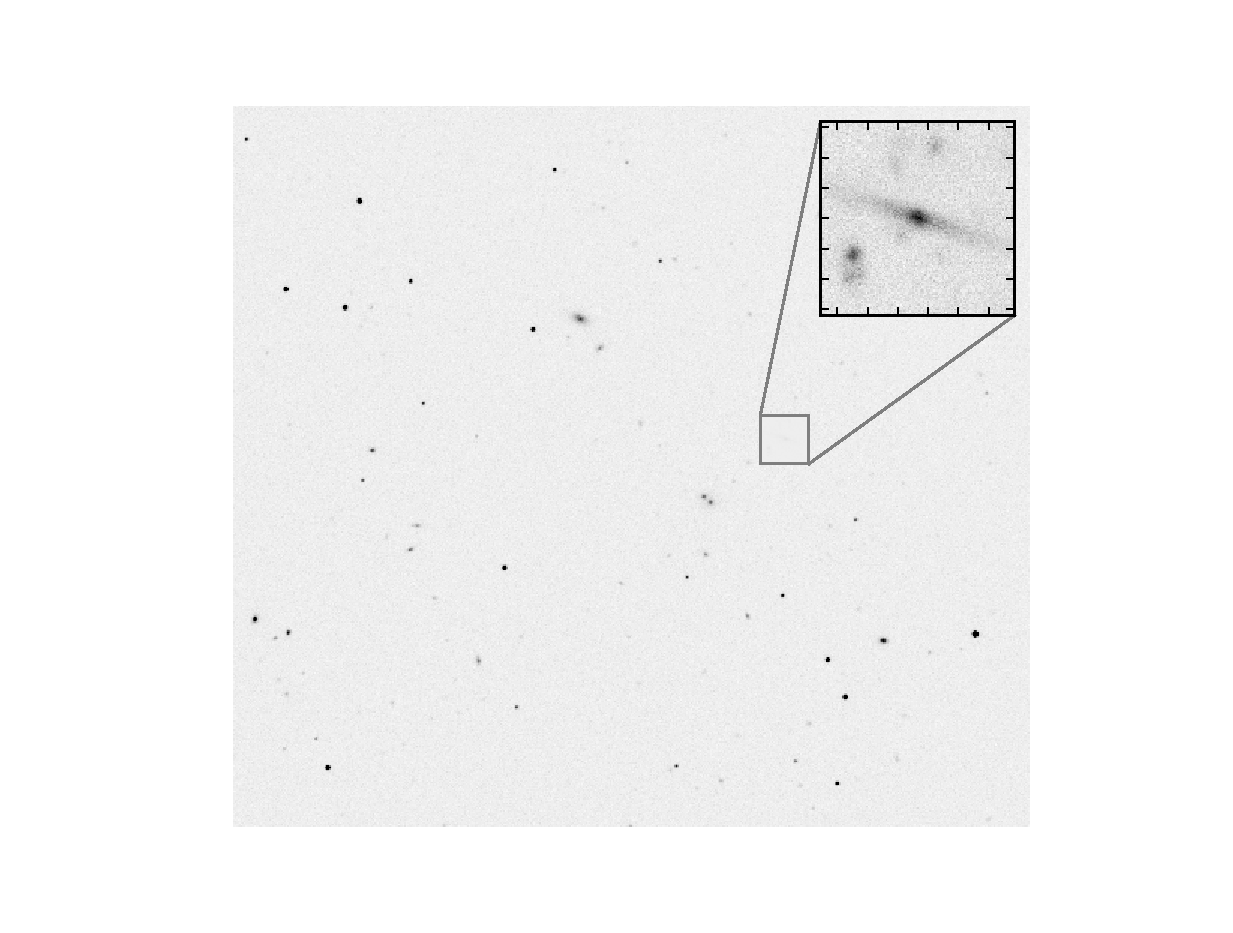
\includegraphics[width=4in,trim=110 50 90 50,clip]{./figures/911to211zoom.eps}
                  \end{minipage} \\
 %               \end{tabular}
%              \end{table}
%\vspace{.5in}
%\begin{center}
            \multicolumn{3}{c}{\begin{minipage}[c][2in][c]{10in}
\textcolor{blue!75!white}{(The data are sequential and low quality).} \end{minipage}} \\
%\end{center}

% before tabular

%\newbox\dhgraphi
%\newbox\dhgraphii
%\newbox\dhgraphiii
%\newbox\dhgraphiv
%\newbox\dhgraphv
%\newbox\dhgraphvi
%\newbox\dhgraphvii
%\newbox\dhgraphviii
%\newbox\dhgraphix
%\newbox\dhgraphx
%\newbox\dhgraphxi
%\newbox\dhgraphxii

%\defgraphUnit{i}{2.5in}{2cm}{$Y_1$}
%\defgraphUnit{ii}{2.5in}{2cm}{$Y_1$}
%\defgraphUnit{ii}{2.5in}{2cm}{$Y_1$}
%\defgraphUnit{ii}{5in}{2cm}{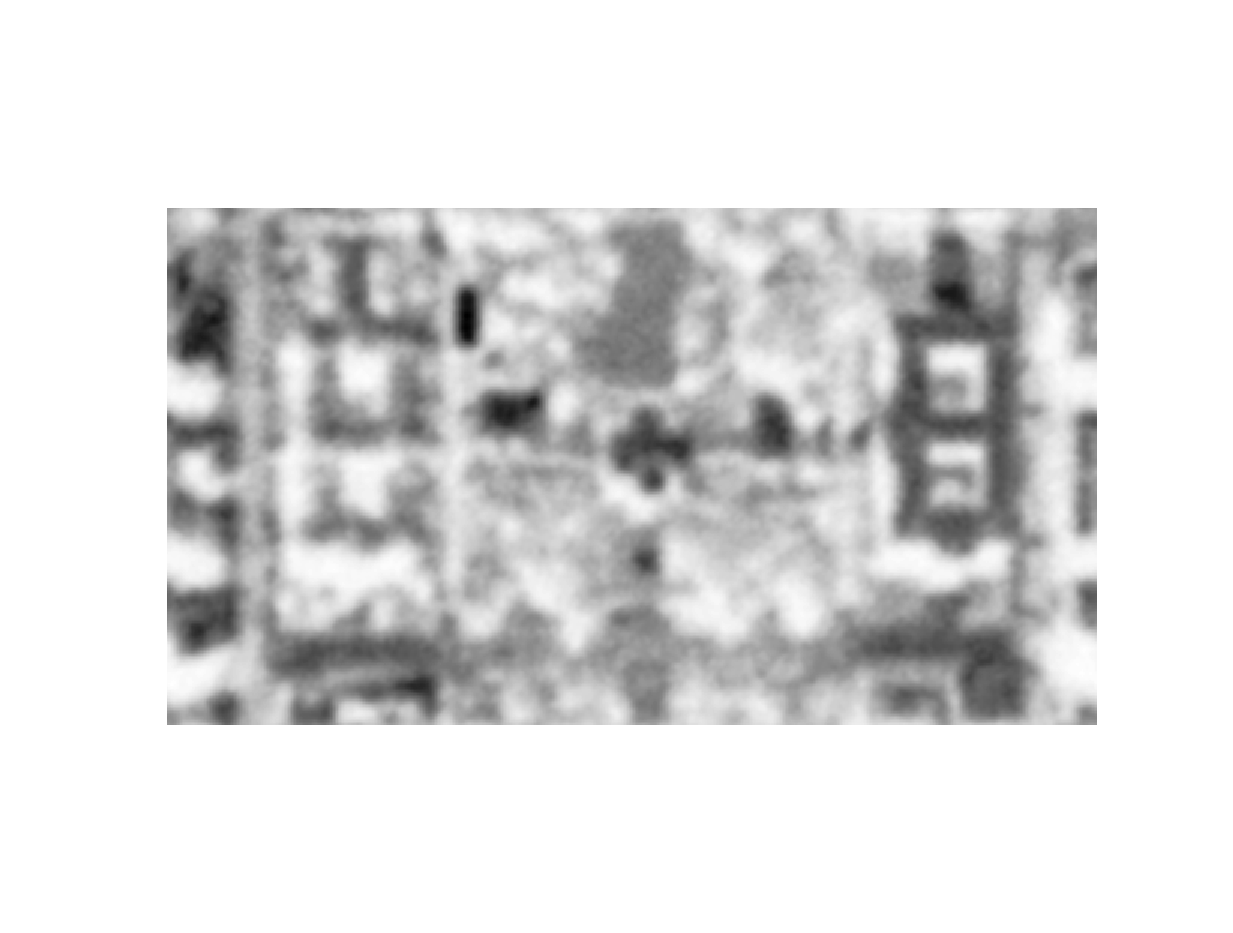
\includegraphics[width=4in,trim=80 130 80 90,clip]{./figures/satelliteAvg1.eps}}
%\defgraphUnit{iii}{5in}{2cm}{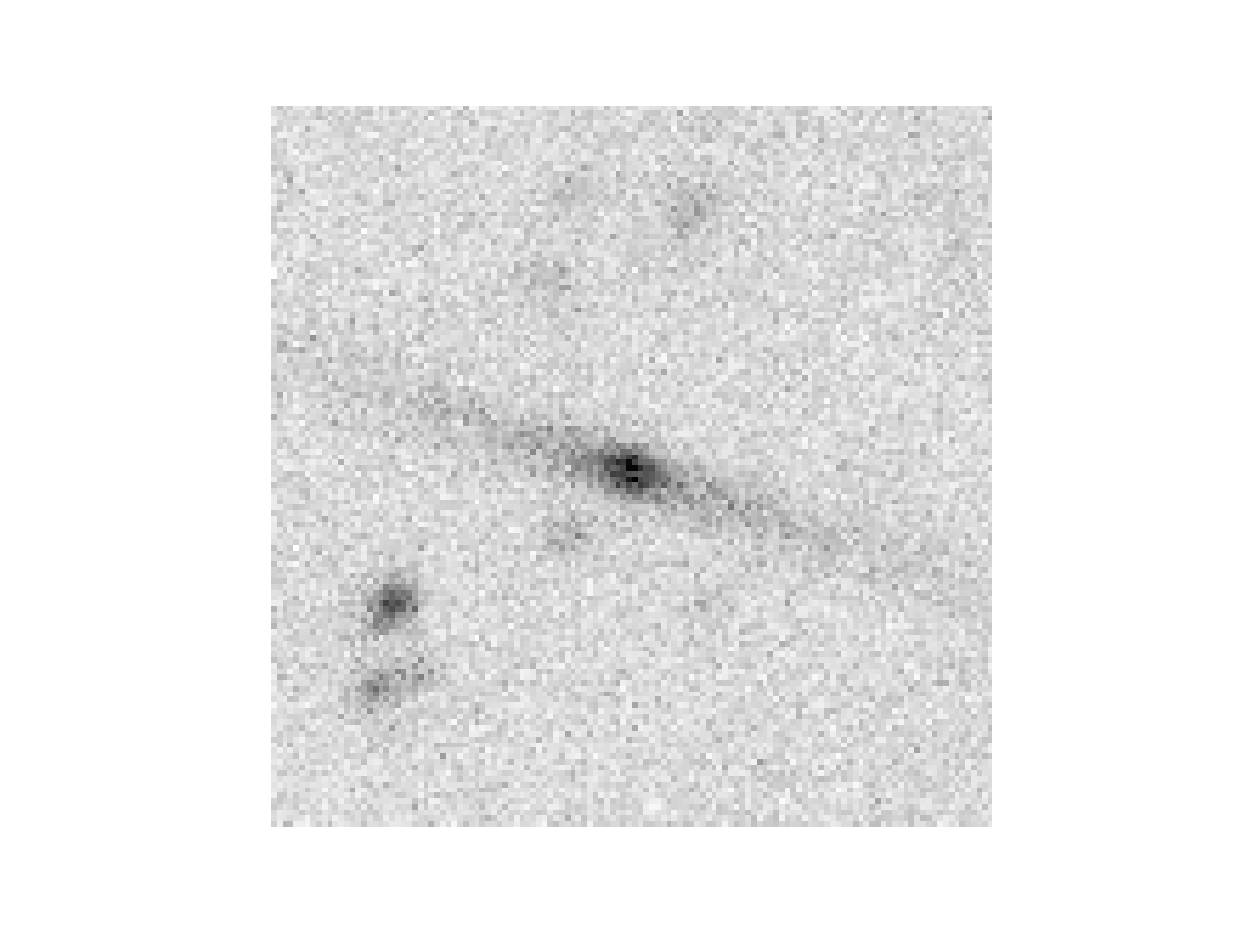
\includegraphics[width=2.5in,trim = 120 50 120 50,clip]{./figures/galaxyPic0.eps}}
%\defgraphUnit{iv}{2.5in}{2cm}{$Y_2$}
%\defgraphUnit{v}{5in}{2cm}{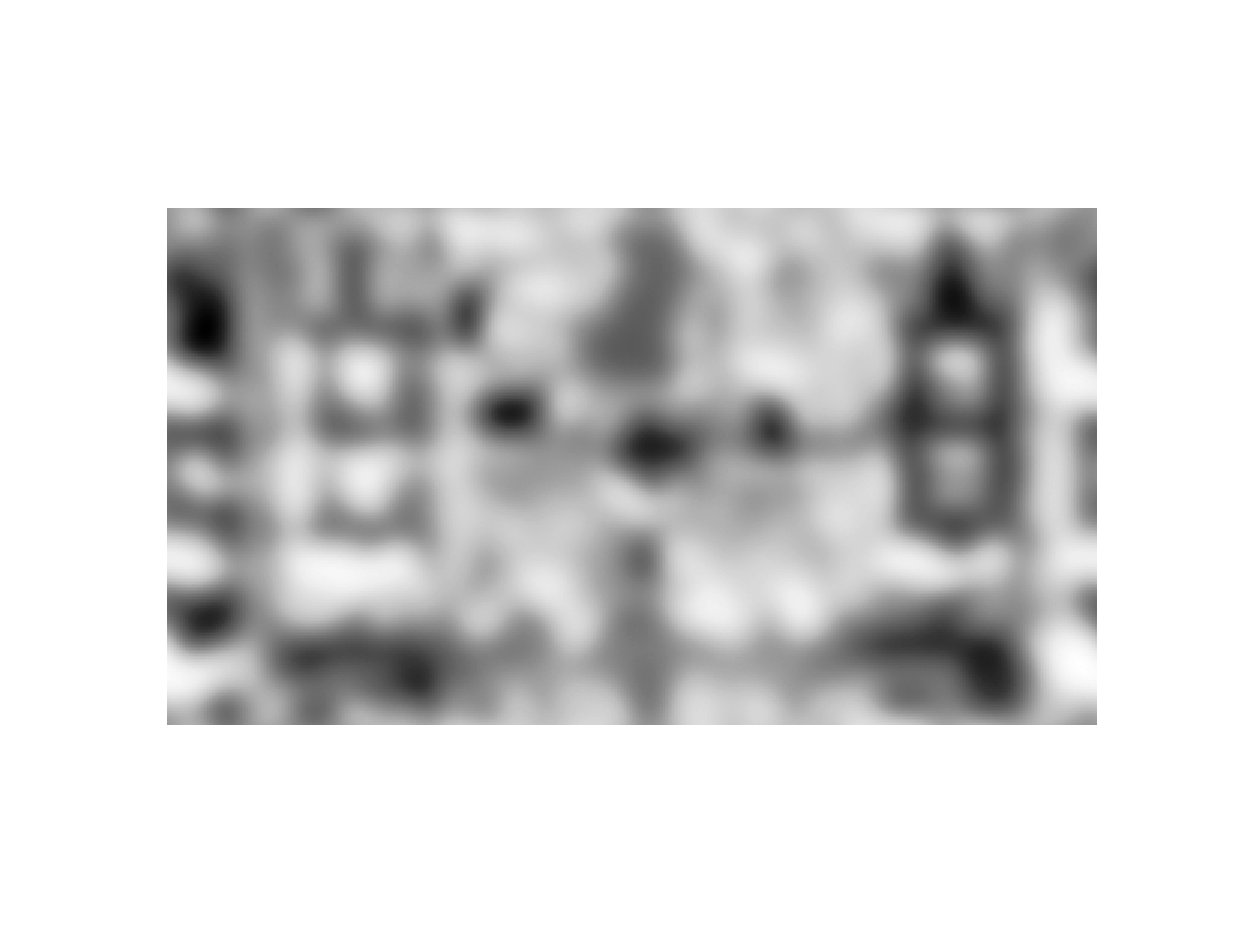
\includegraphics[width=4in,trim=80 130 80 90,clip]{./figures/satelliteWorst.eps}}
%\defgraphUnit{vi}{5in}{2cm}{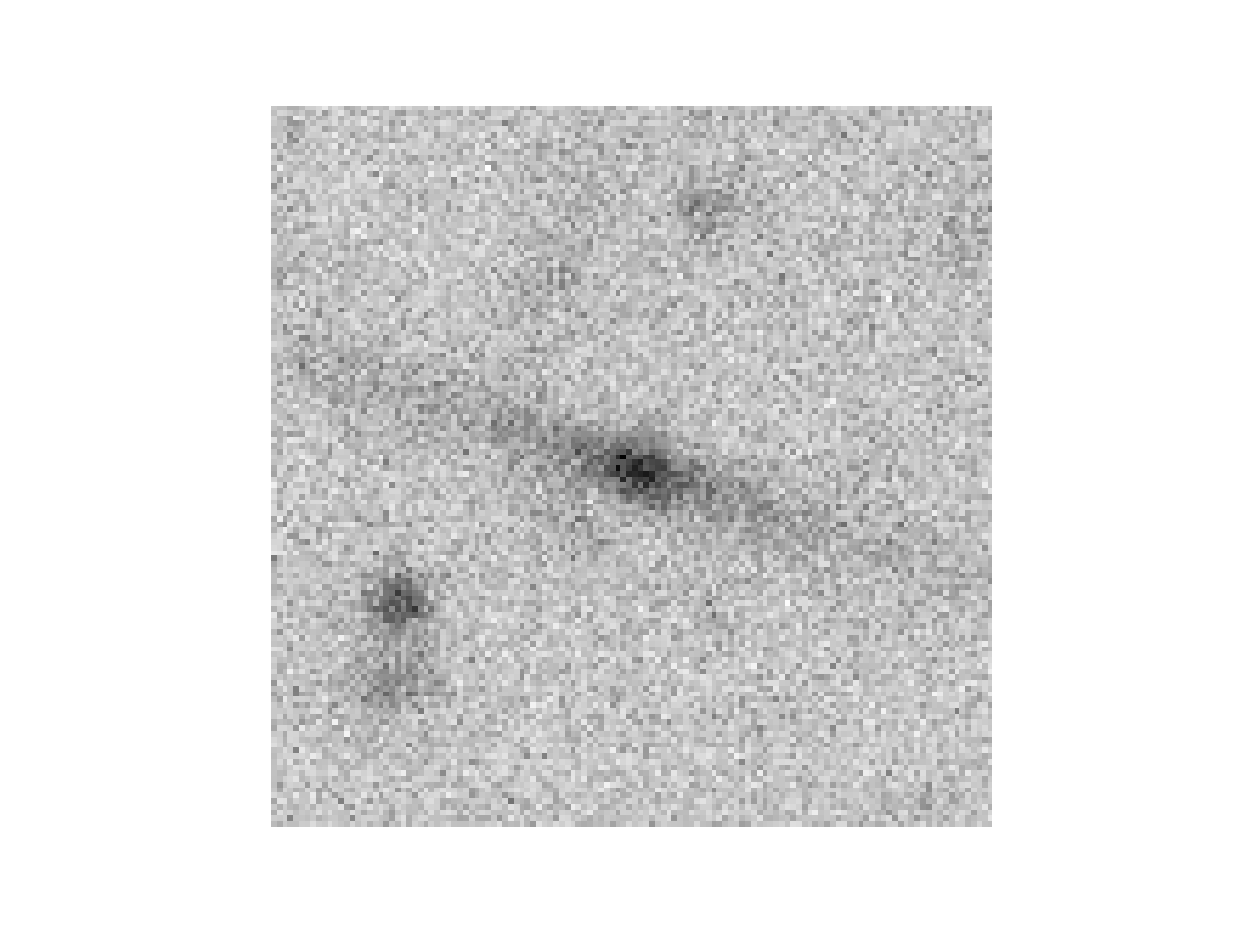
\includegraphics[width=2.5in,trim = 120 50 120 50,clip]{./figures/galaxyPic1.eps}}
%\defgraphUnit{vii}{2.5in}{2cm}{$Y_3$}
%\defgraphUnit{viii}{5in}{2cm}{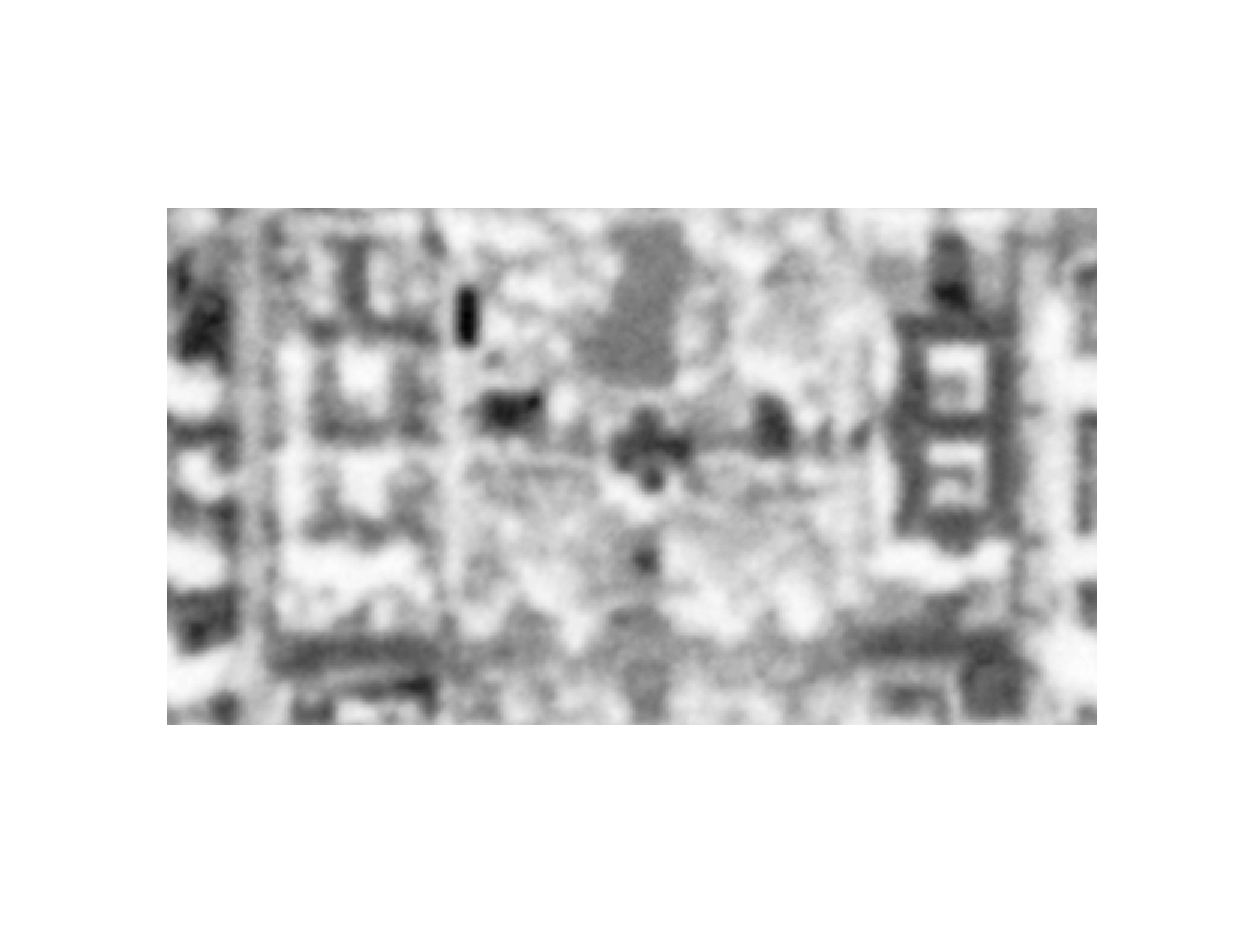
\includegraphics[width=4in,trim=80 130 80 90,clip]{./figures/satelliteAvg2.eps}}
%\defgraphUnit{ix}{5in}{2cm}{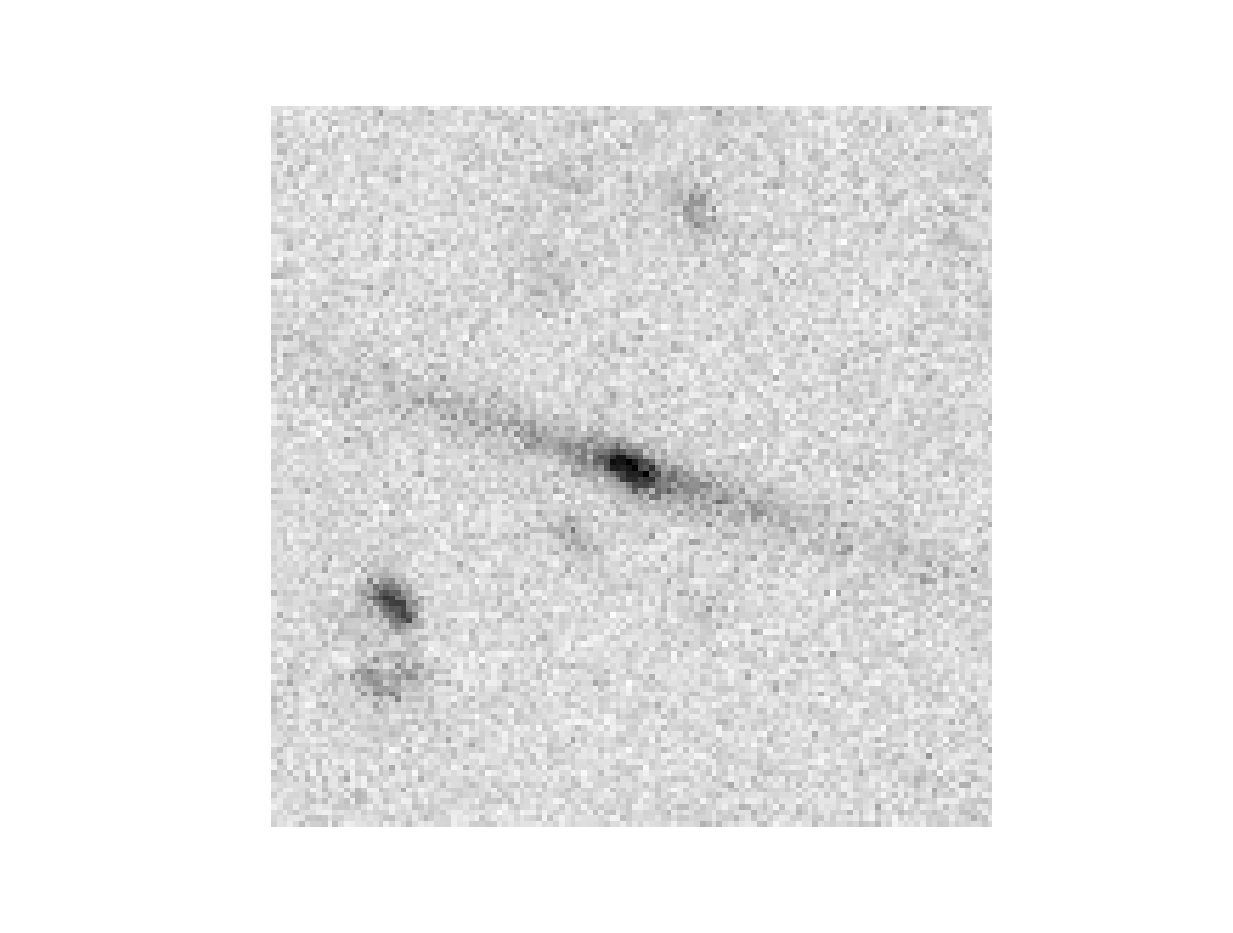
\includegraphics[width=2.5in,trim = 120 50 120 50,clip]{./figures/galaxyPic2.eps}}
%\defgraphUnit{x}{2.5in}{2cm}{$Y_2$}
%\defgraphUnit{xi}{5in}{2cm}{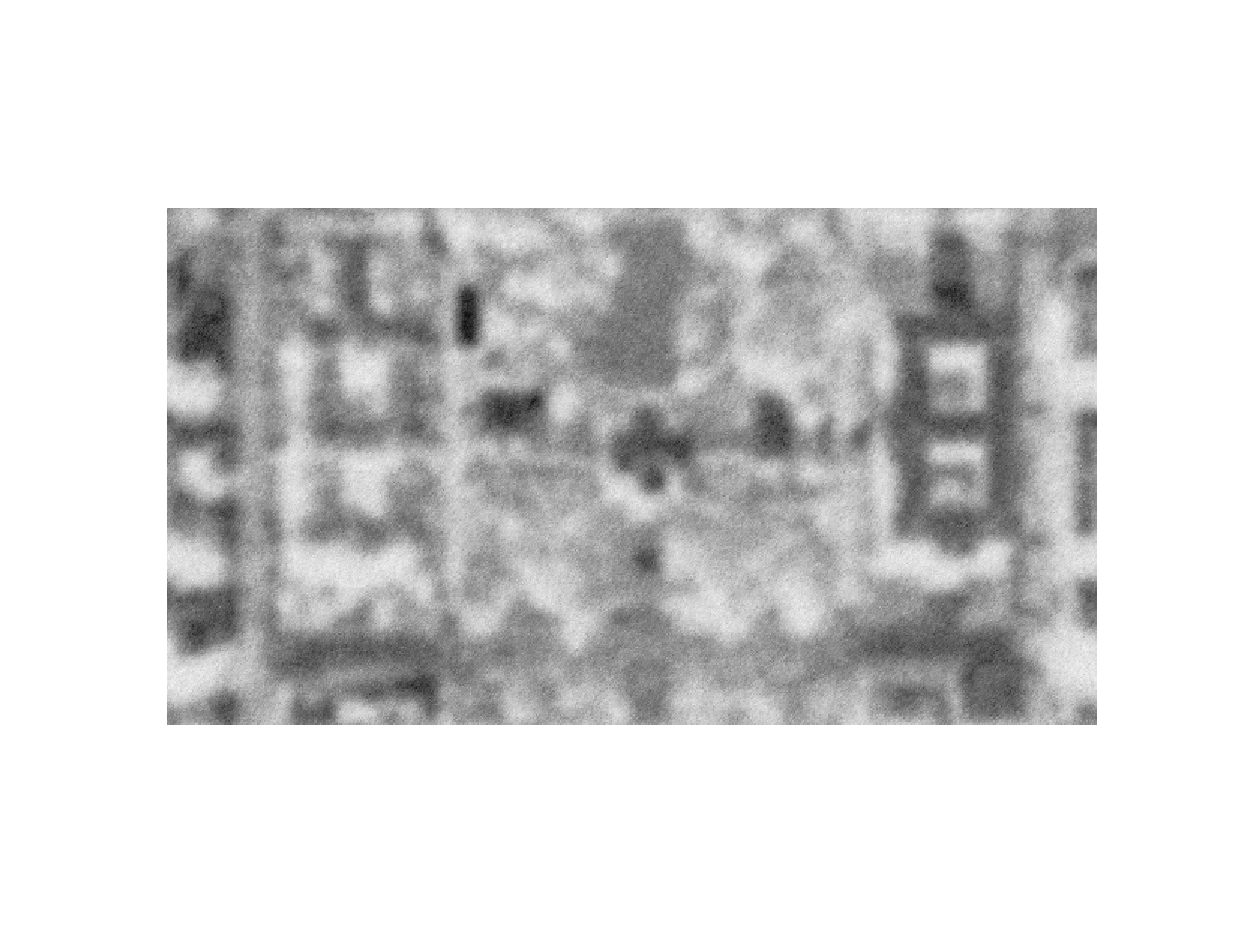
\includegraphics[width=4in,trim=80 130 80 90,clip]{./figures/satelliteBest.eps}}
%\defgraphUnit{xii}{5in}{2cm}{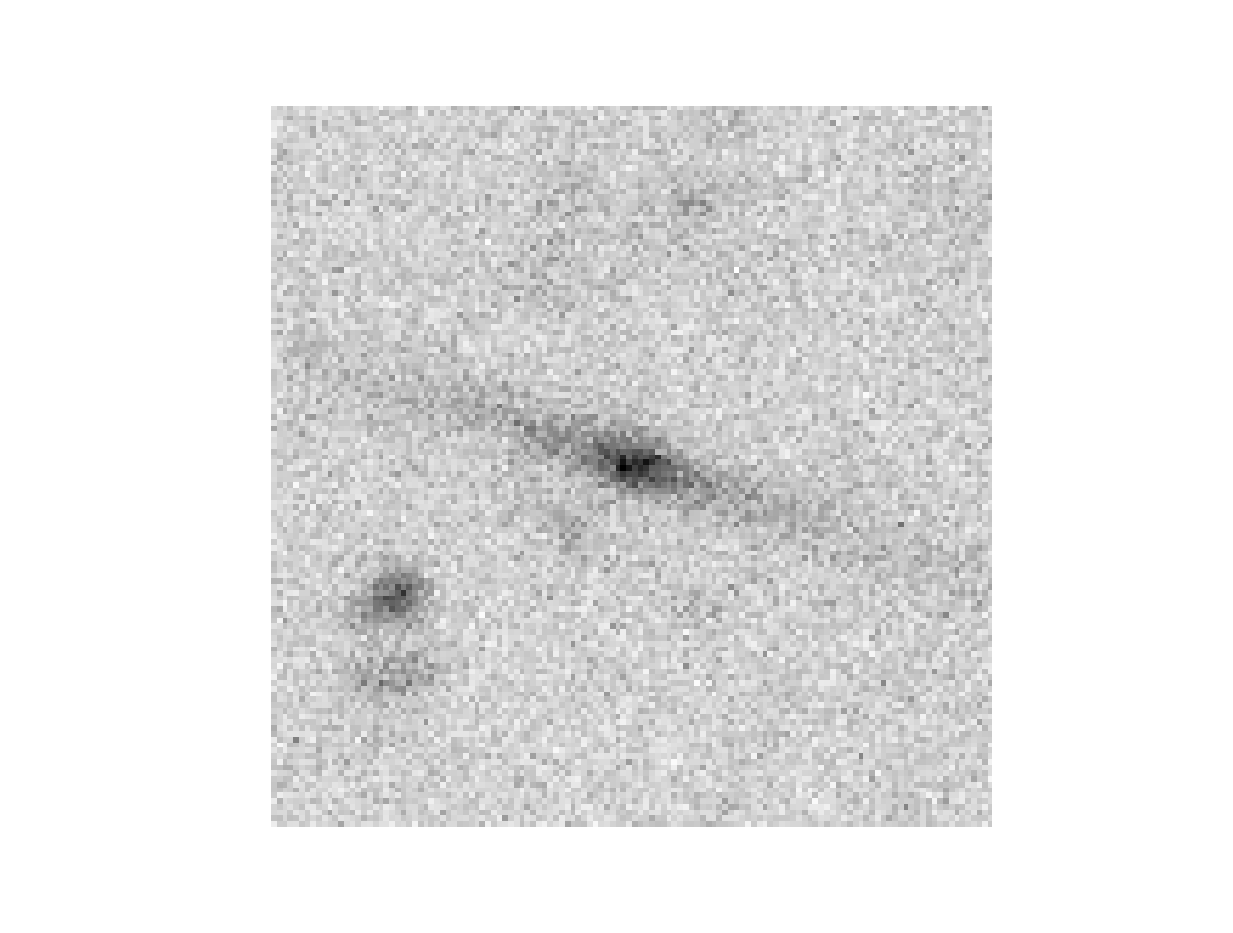
\includegraphics[width=2.5in,trim = 120 50 120 50,clip]{./figures/galaxyPic3.eps}}

% in tabular

%\def\graphRow#1#2#3{\box\csname dhgraph#1\endcsname&\box\csname dhgraph#2\endcsname&\box\csname dhgraph#3\endcsname}

%\graphRow{i}{ii}{iii}\\
%\graphRow{iv}{v}{vi}\\
%\graphRow{vii}{viii}{ix}\\
%\graphRow{x}{xi}{xii}\\


%              \begin{table}
%                \centering
%                \begin{tabular}{ccc}
                  \begin{minipage}[r][2.5in][c]{3cm}
                    $Y_1$
                  \end{minipage} &
                  \begin{minipage}[c][2.5in][c]{6in}
                    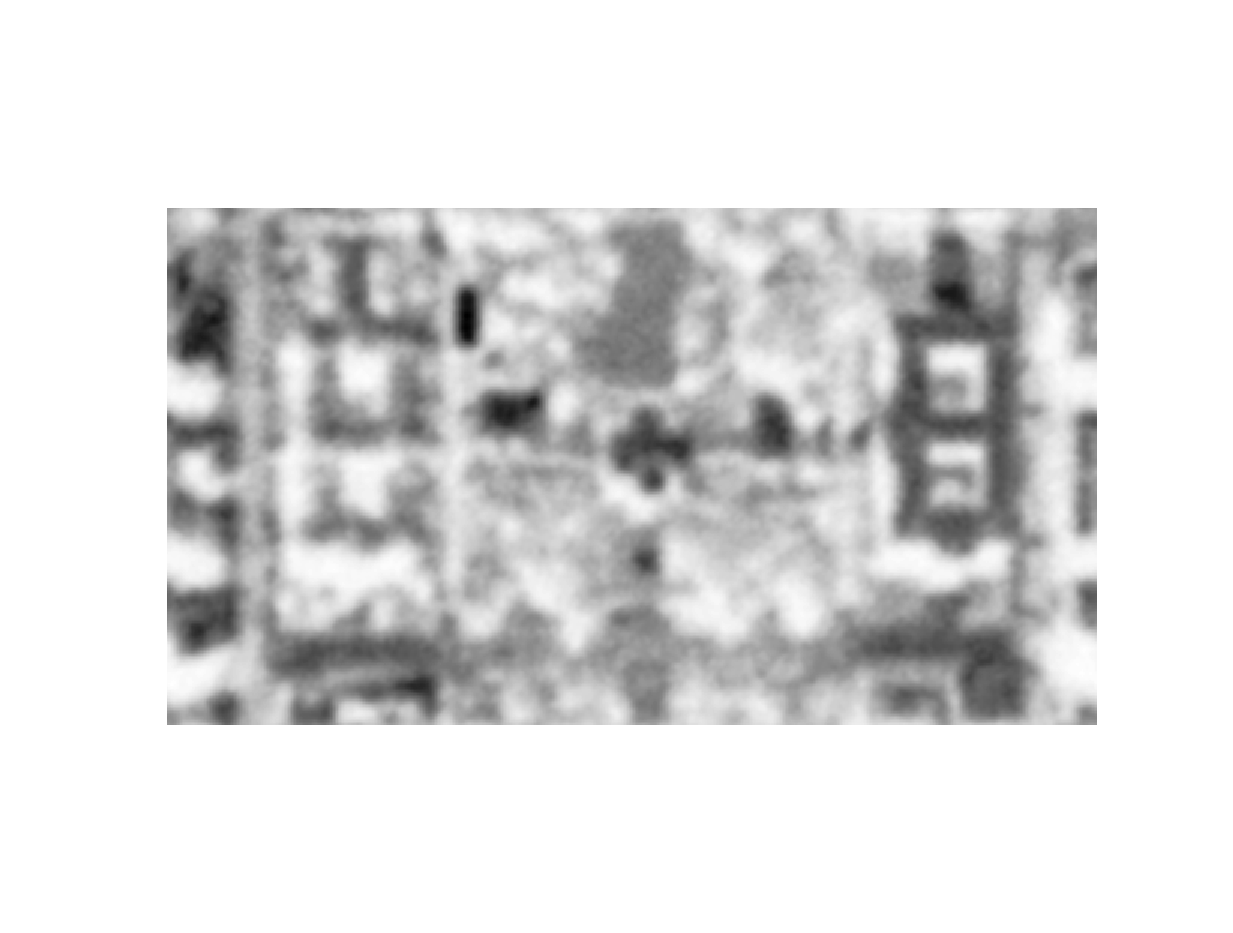
\includegraphics[width=5in,trim=80 130 80 90,clip]{./figures/satelliteAvg1.eps}
                  \end{minipage} &
                  \begin{minipage}[c][2.5in][c]{5in}
                    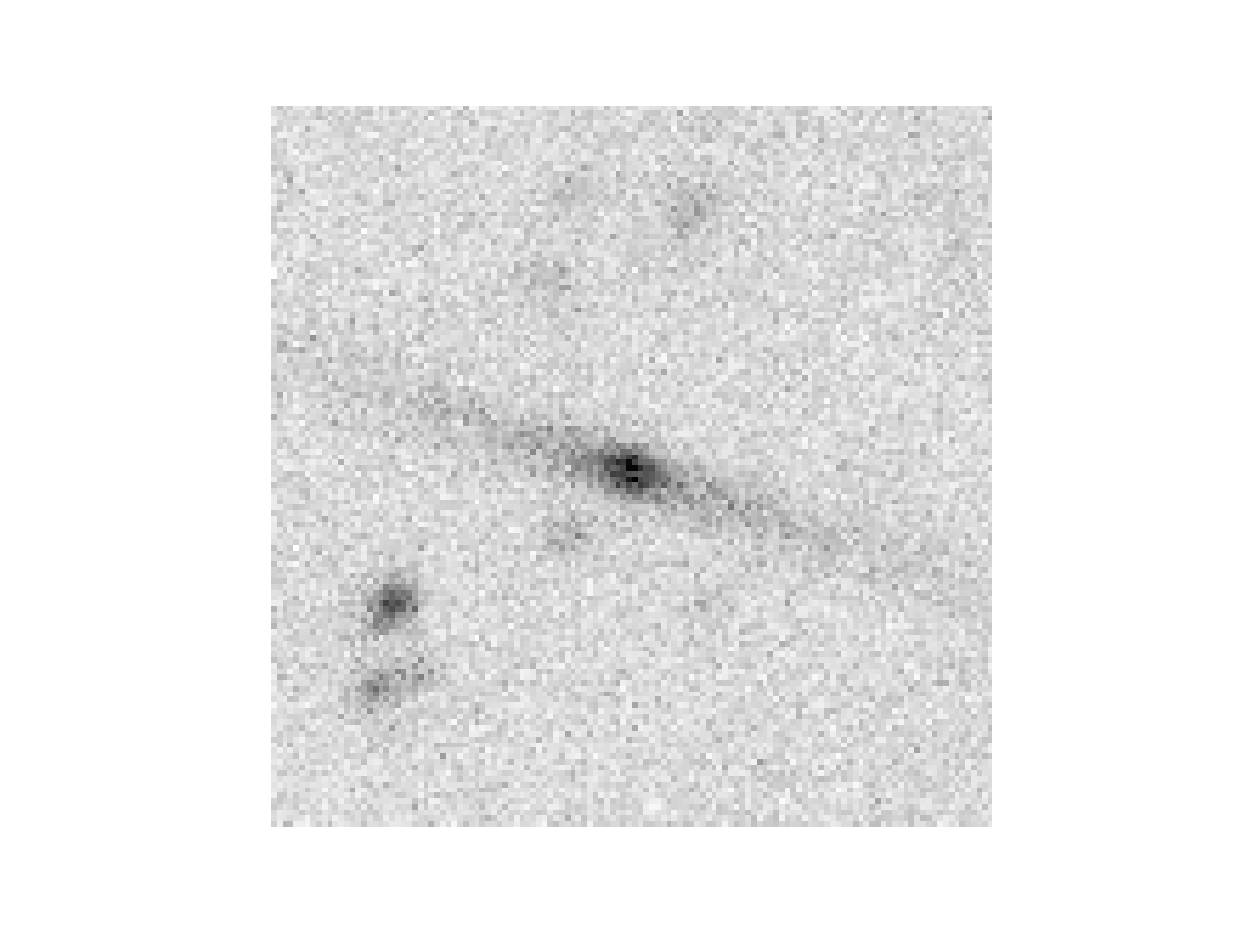
\includegraphics[width=2.7in,trim = 120 50 120 50,clip]{./figures/galaxyPic0.eps}
                  \end{minipage} 
                  \\
                  \begin{minipage}[c][2.5in][c]{3cm}
                    $Y_2$
                  \end{minipage} &
                  \begin{minipage}[c][2.5in][c]{6in}
                    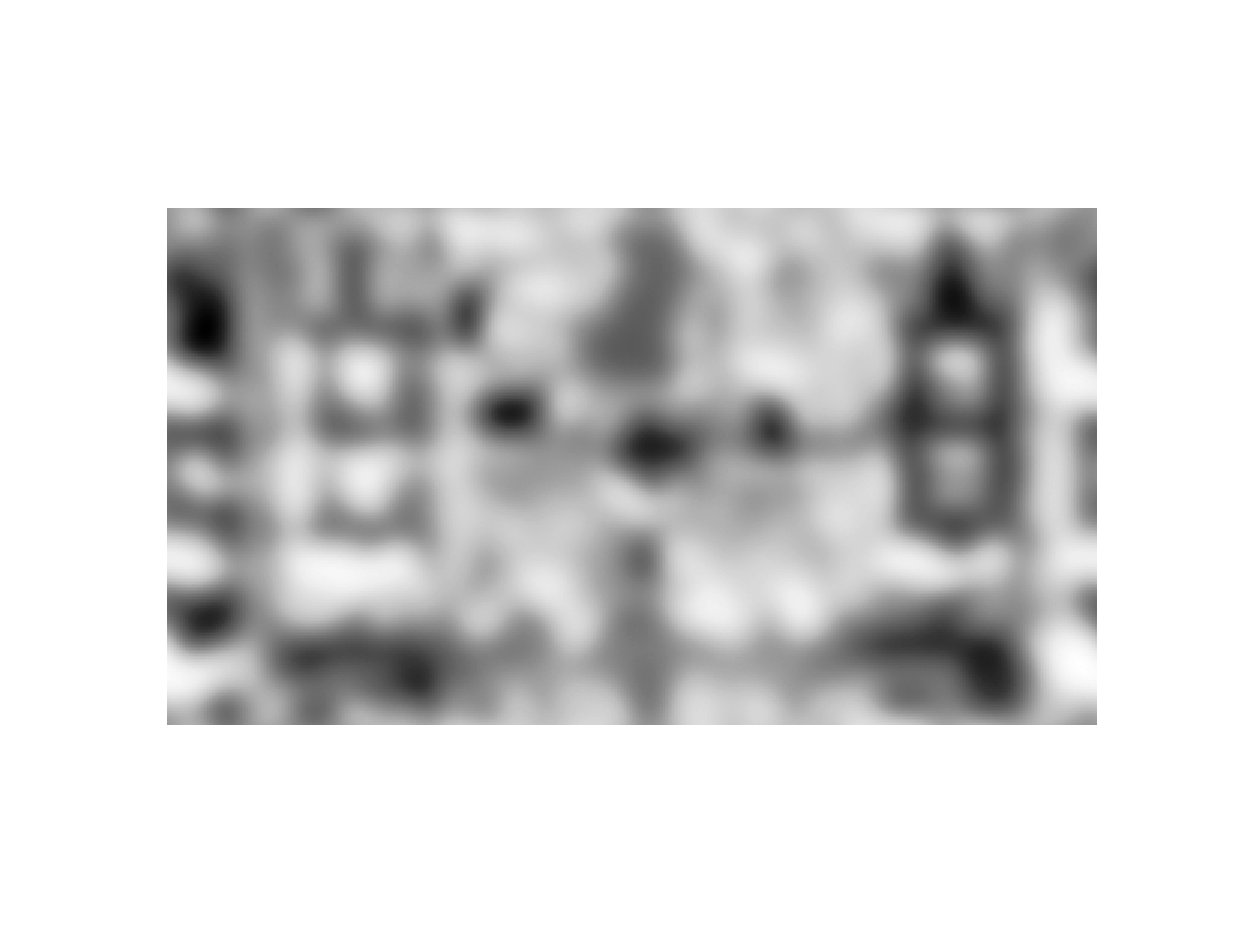
\includegraphics[width=5in,trim=80 130 80 90,clip]{./figures/satelliteWorst.eps}
                  \end{minipage} &
                  \begin{minipage}[c][2.5in][c]{5in}
                    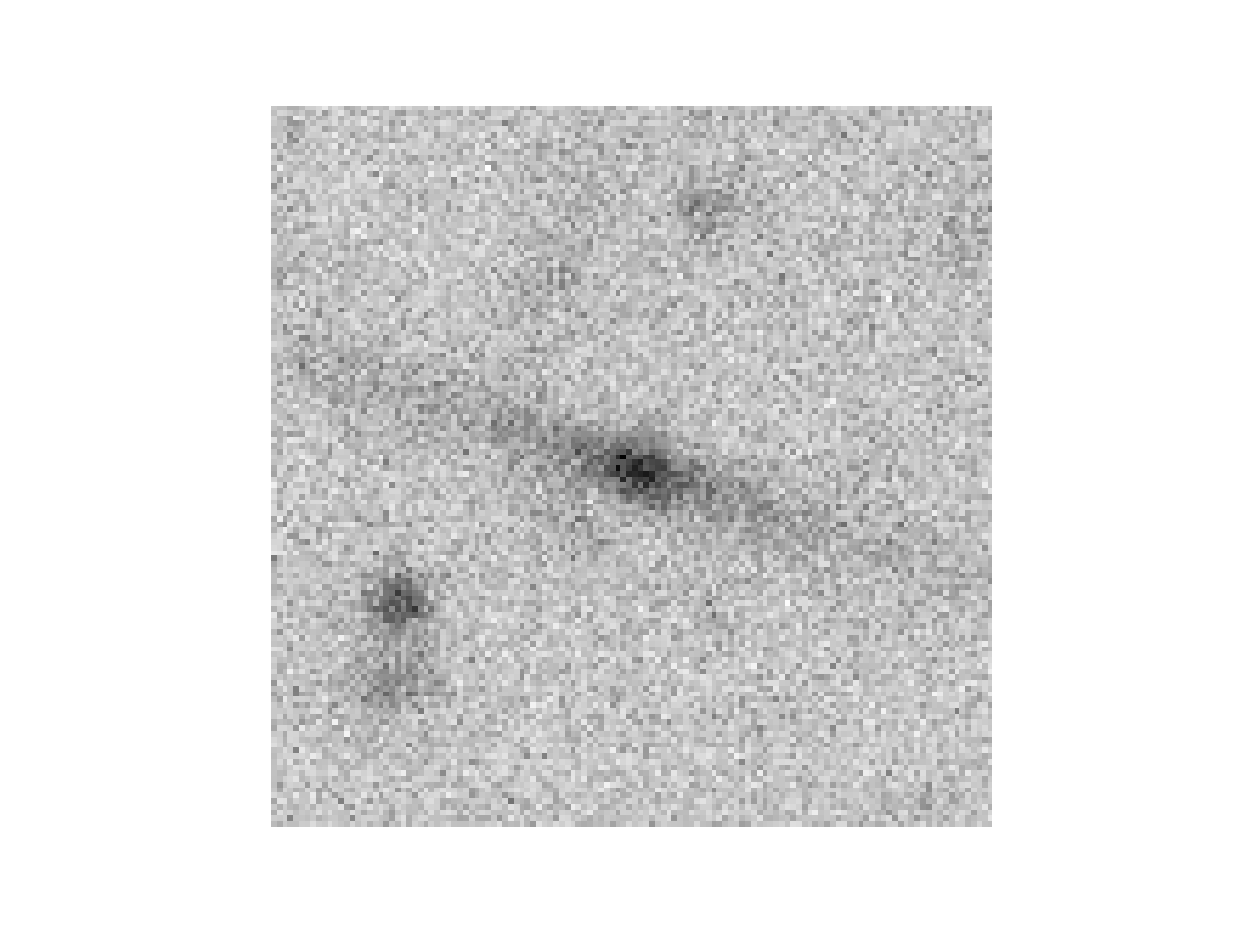
\includegraphics[width=2.7in,trim = 120 50 120 50,clip]{./figures/galaxyPic1.eps}
                  \end{minipage} \\
                  \begin{minipage}[c][2.5in][c]{3cm}
                    $Y_3$
                  \end{minipage} &
                  \begin{minipage}[c][2.5in][c]{6in}
                    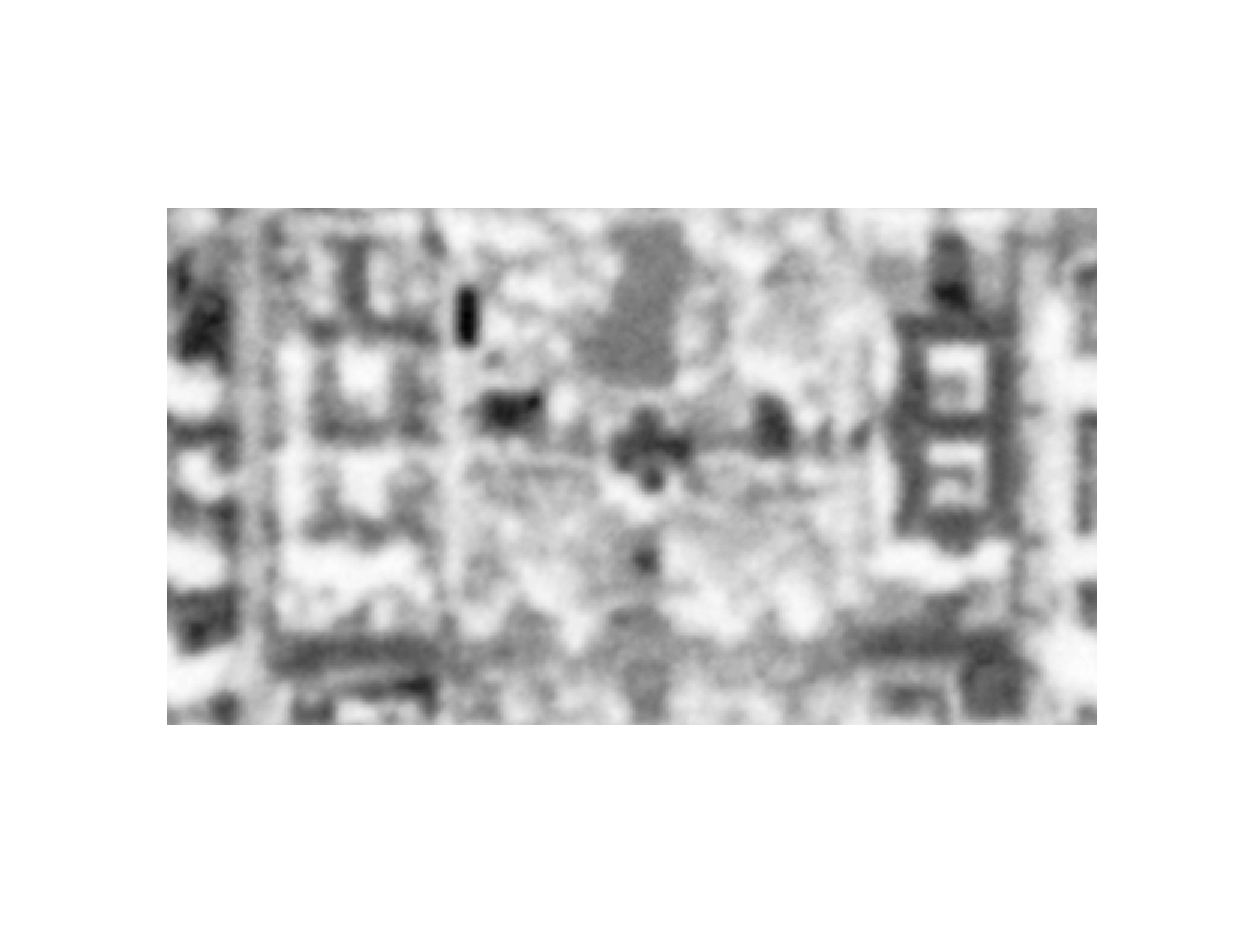
\includegraphics[width=5in,trim=80 130 80 90,clip]{./figures/satelliteAvg2.eps}
                  \end{minipage} &
                  \begin{minipage}[c][2.5in][c]{5in}
                    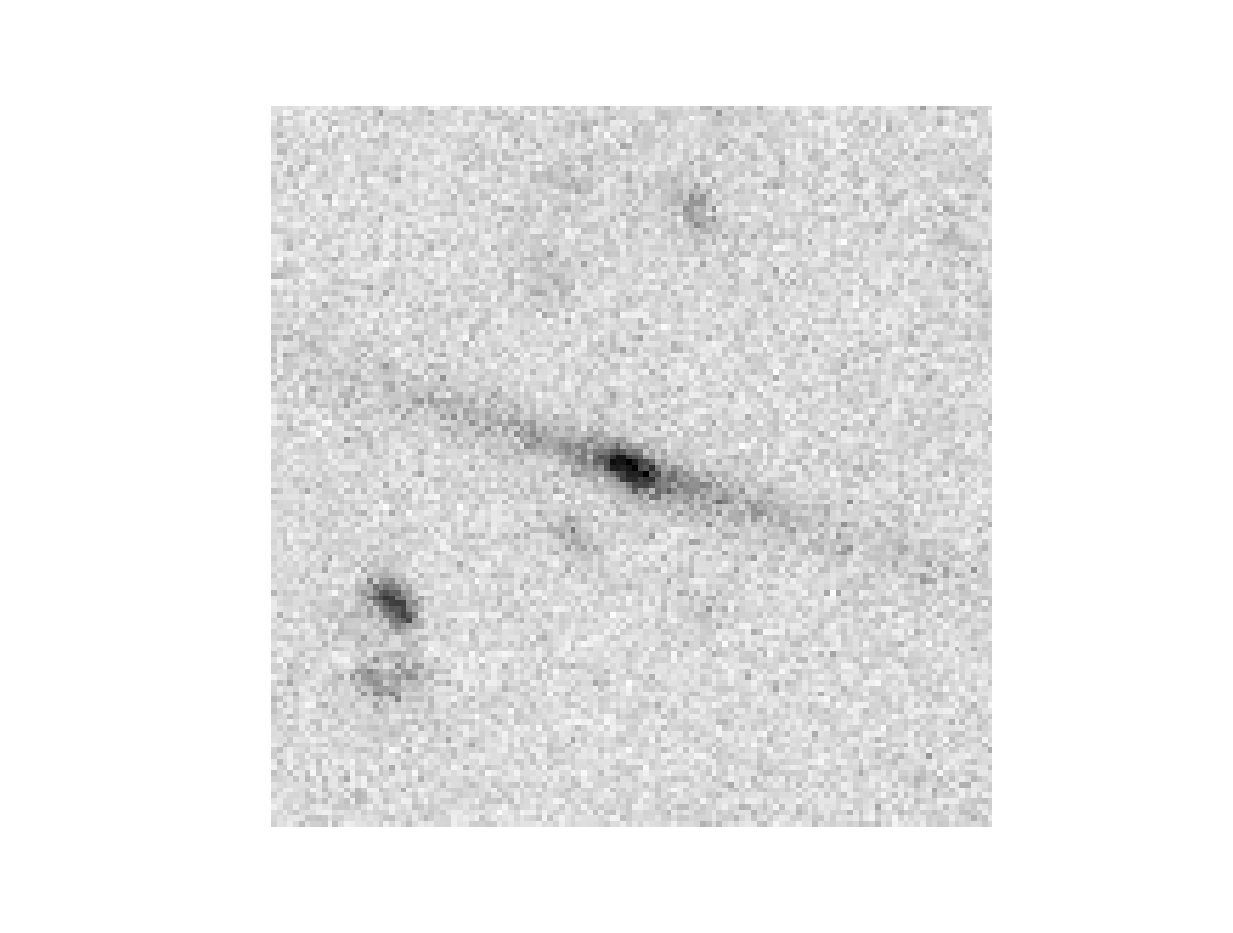
\includegraphics[width=2.7in,trim = 120 50 120 50,clip]{./figures/galaxyPic2.eps}
                  \end{minipage} \\
                  \begin{minipage}[c][2.5in][c]{3cm}
                    $Y_2$
                  \end{minipage} &
                  \begin{minipage}[c][2.5in][c]{6in}
                    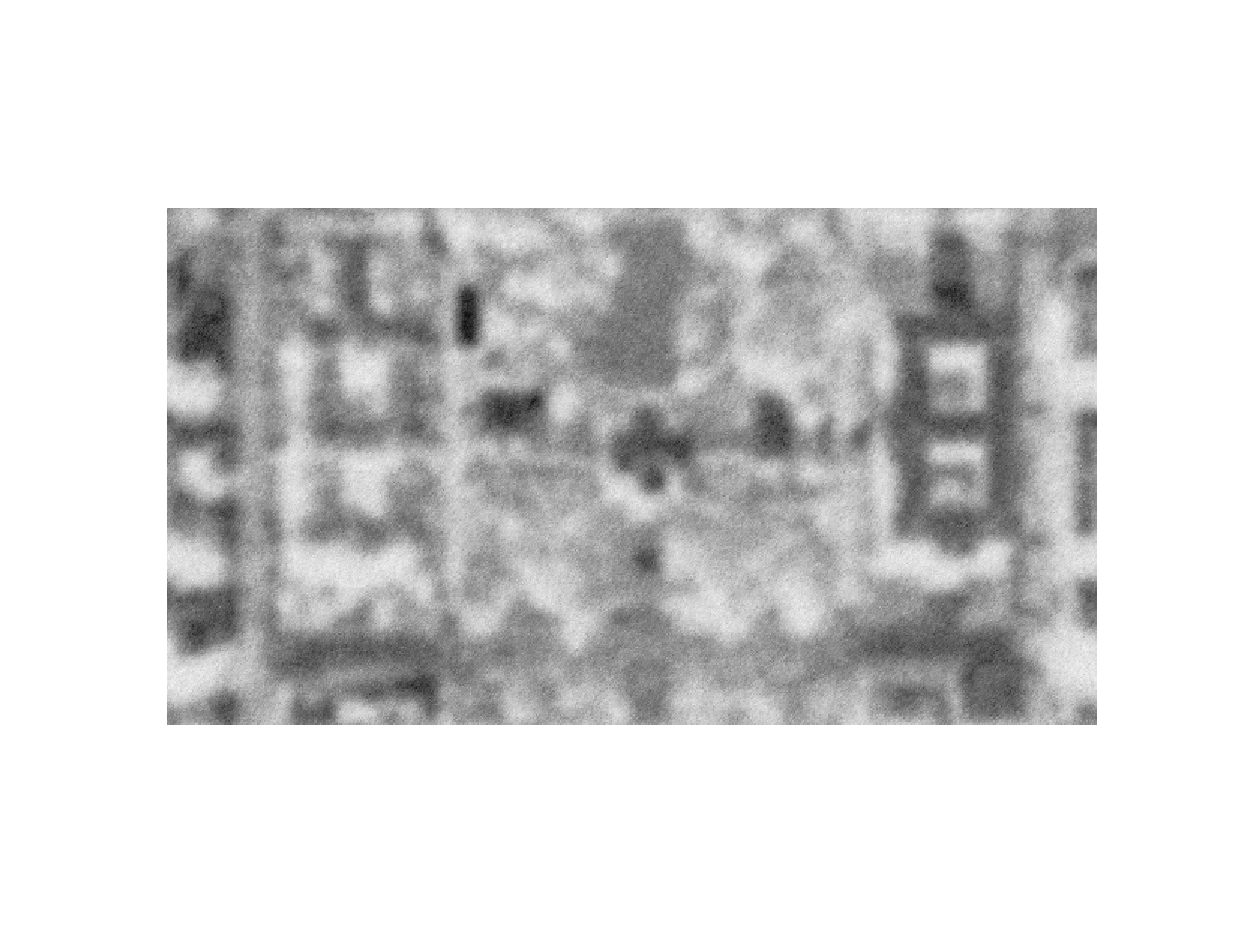
\includegraphics[width=5in,trim=80 130 80 90,clip]{./figures/satelliteBest.eps}
                  \end{minipage} &
                  \begin{minipage}[r][2.5in][r]{5in}
                    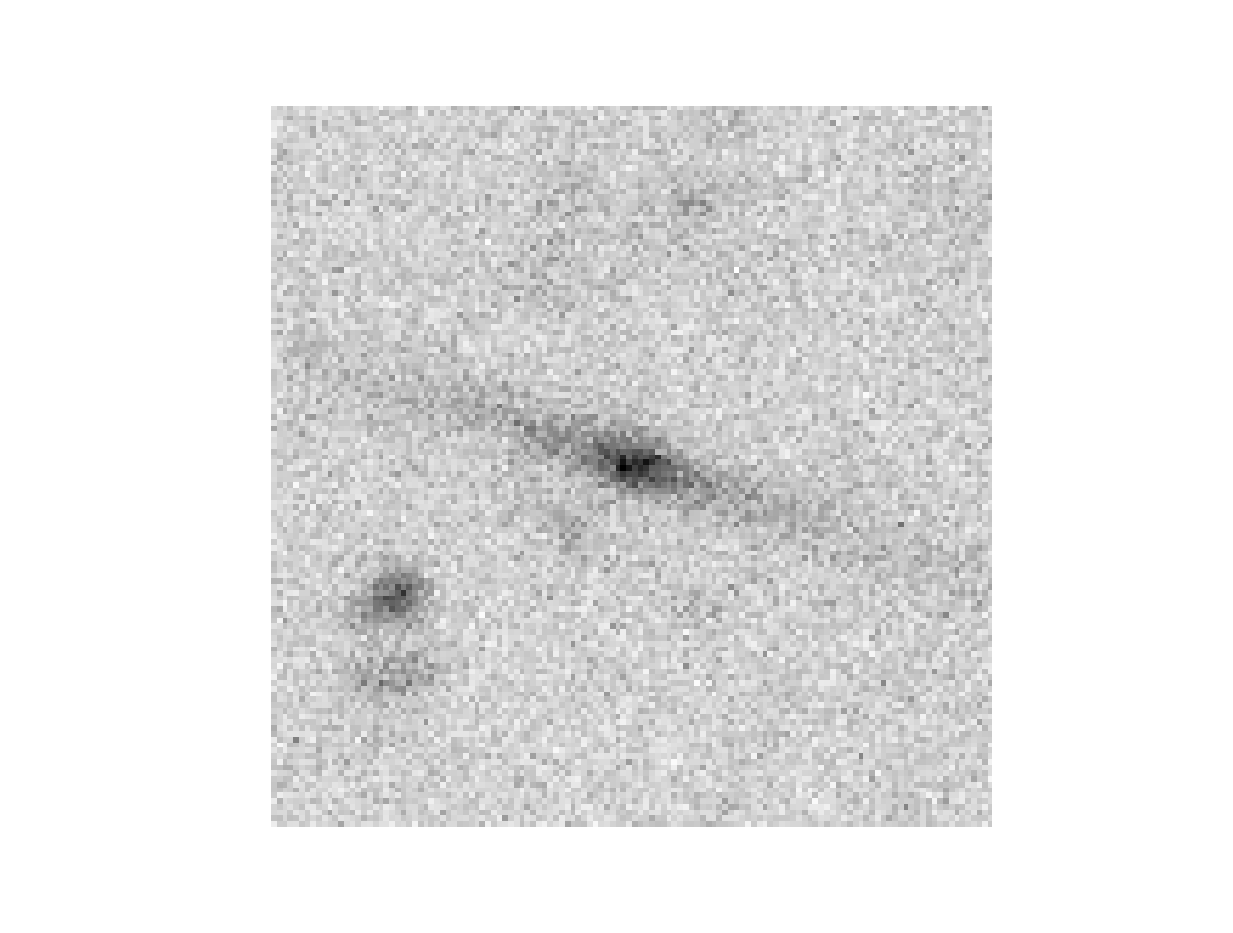
\includegraphics[width=2.7in,trim = 120 50 120 50,clip]{./figures/galaxyPic3.eps}
                  \end{minipage}
                \end{tabular}
              \end{table}
            \end{block} 
            \begin{block}{Reconstruction with Our Estimator:}
              \begin{table}
                \centering
                \begin{tabular}{ccc}
%                  \begin{minipage}[c][1.5in][c]{3cm}
%                    After: 
%                  \end{minipage} &
 %                 \begin{minipage}[c][1.5in][c]{6in}
%                    $n = 4$ observations
%                  \end{minipage} &
%                  \begin{minipage}[c][1.5in][c]{6in}
 %                   $n = 12$ observations
 %%                 \end{minipage} \\
                  \begin{minipage}[c][2.5in][c]{3cm}
                  $\hat\theta_n$ 
                  \end{minipage} &
                  \begin{minipage}[c][2.5in][c]{6in}
                  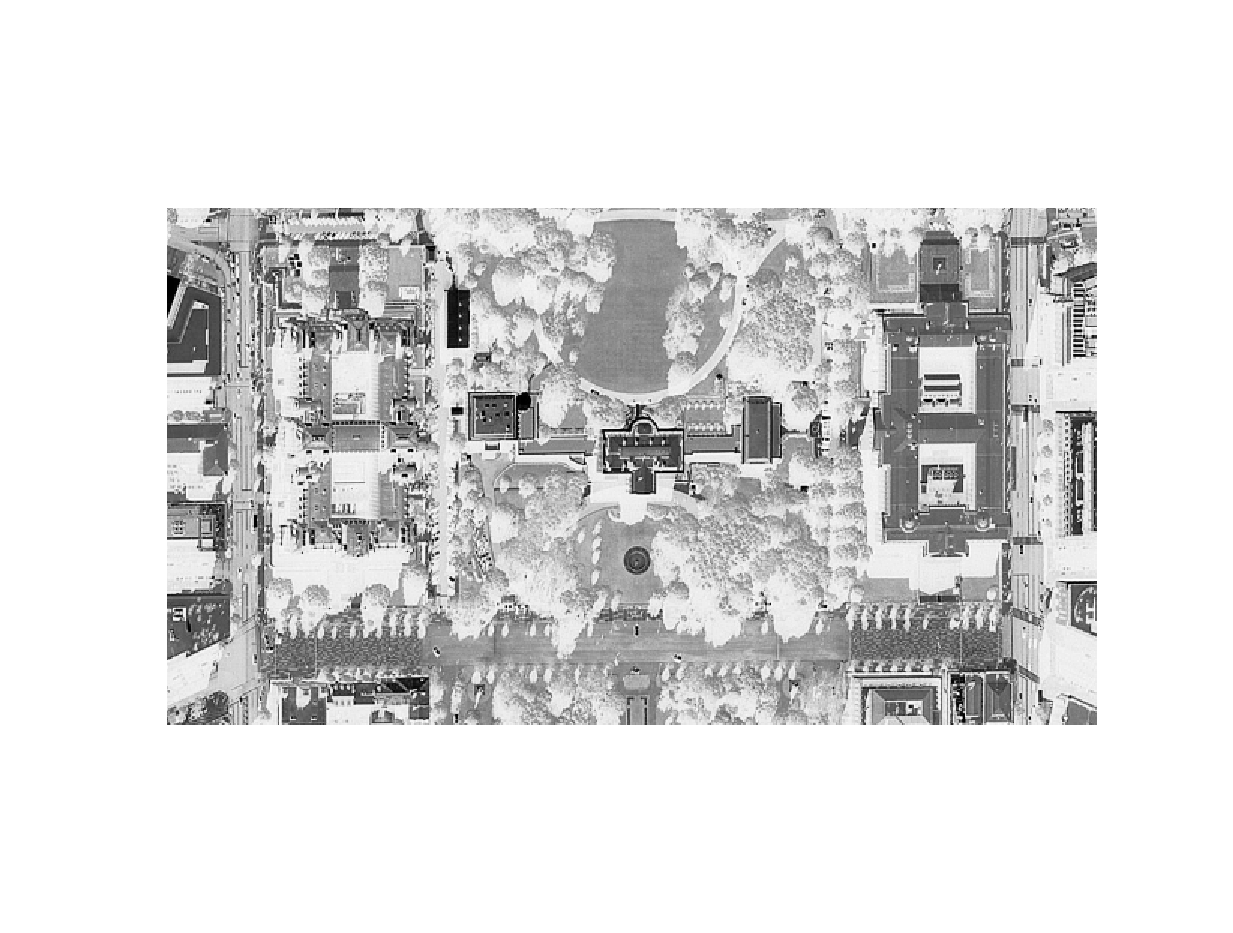
\includegraphics[width = 5in,trim=80 130 80 90,clip]{./figures/satelliteEstimator4.eps} 
                  \end{minipage} &
                  \begin{minipage}[c][2.5in][c]{5in}
                  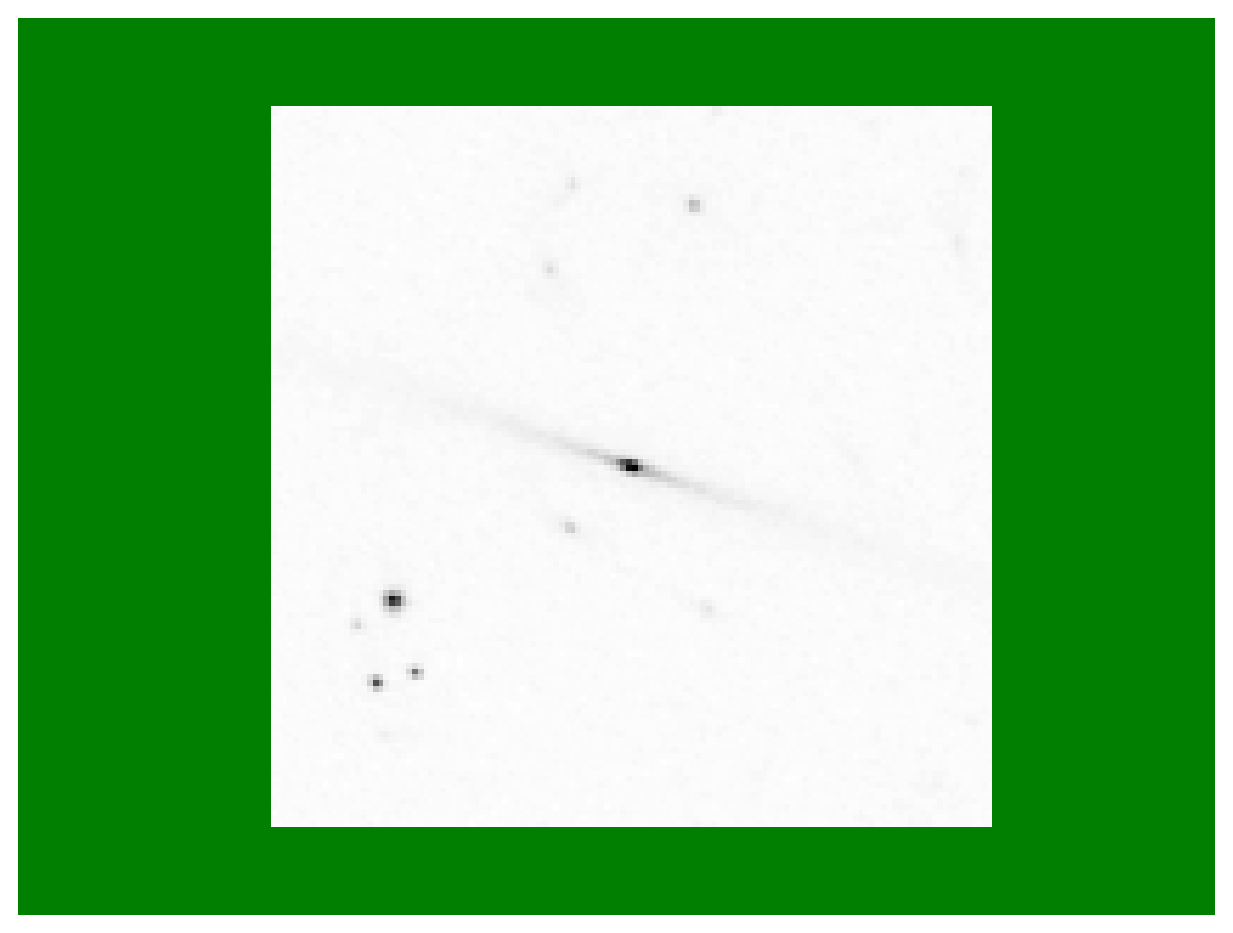
\includegraphics[width=2.7in,trim = 120 40 105 40,clip]{./figures/astroEstimator4green.eps} 
                  \end{minipage}
                \end{tabular}
              \end{table}
            \end{block}
          % 
          \vfill
          % 
          }
        \end{minipage}
      \end{beamercolorbox}
    \end{column}
%  % 
%  % 
%  % Column 2
%  % 
%  % 
  \begin{column}{.32\textwidth}
    \begin{beamercolorbox}[center,wd=\textwidth]{postercolumn}
      \begin{minipage}[T]{.95\textwidth} 
        \parbox[t][\columnheight]{\textwidth}{
          % 
          \vfill
          % 
            \begin{alertblock}{Scientific Goals}
              Formulate an estimator that:
              \begin{itemize}
              \item Has good theoretical properties.
              \item Requires no user defined tuning parameters.
              \item Can be efficiently updated after recording a new observation.
              \end{itemize}
            \end{alertblock}
          % 
          \vfill
          % 
          \begin{block}{Statistical Model:}
For $i = 1,\ldots,n,\ldots$
\[
Y_i = K_i\theta + \epsilon Z_i
\]
\end{block}
\begin{block}{Assumptions:}
\begin{itemize}
\item[1.] $\displaystyle{\theta \in \Theta = \{\theta : ||\theta ||_2^2 \leq T^2, \theta \in \mathbb{R}^p\}}$. \\
\item[2.] $\epsilon$ is known 
\item[] Suppose $(K_i)_{i=1}^n$ are
  \begin{itemize}
    \item[3a.] Known
    \item[3b.] Simultaneously diagonalizable \\
    ($\exists$ unitary $\Psi \in \mathbb{C}^{p\times p}$ s.t. $K_i = \Psi D_i \Psi^*$ for some diagonal $D_i$).
      \begin{itemize}
        \item[] \textcolor{blue!75!white}{(This includes circulant matrices and hence convolutions.)}
      \end{itemize}
  \end{itemize}
\end{itemize}
          \end{block}
\begin{block}{Manipulations:}
Begin by rotating by eigenvectors $\Psi$:
\begin{itemize}
\item $\beta := \Psi^* \theta \in \mathbb{C}^p$.
\item $\mathcal{B} := \Psi^* \Theta$
\item $X_i := \Psi^* Y_i$
\end{itemize}
Define 
\begin{itemize}
\item $\displaystyle{\Delta_n := \sum_{i=1}^n D_i^*D_i = \sum_{i=1}^n |D_i|^2}$
\item $B_n = \Delta_n^{-1}\sum_{i=1}^n D_i^*X_i $
\end{itemize}

%\begin{propo}
%The random vector $\mathbf{B}_n = \Delta_n^{-1}\sum_{i=1}^n D_i^*X_i $
%is sufficient for $\beta$.
%\end{propo}

%Example: Why $\Psi\mathbf{B}_n$ cannot be used as an estimator
%\begin{table}
%\centering
%\begin{tabular}{cc}
%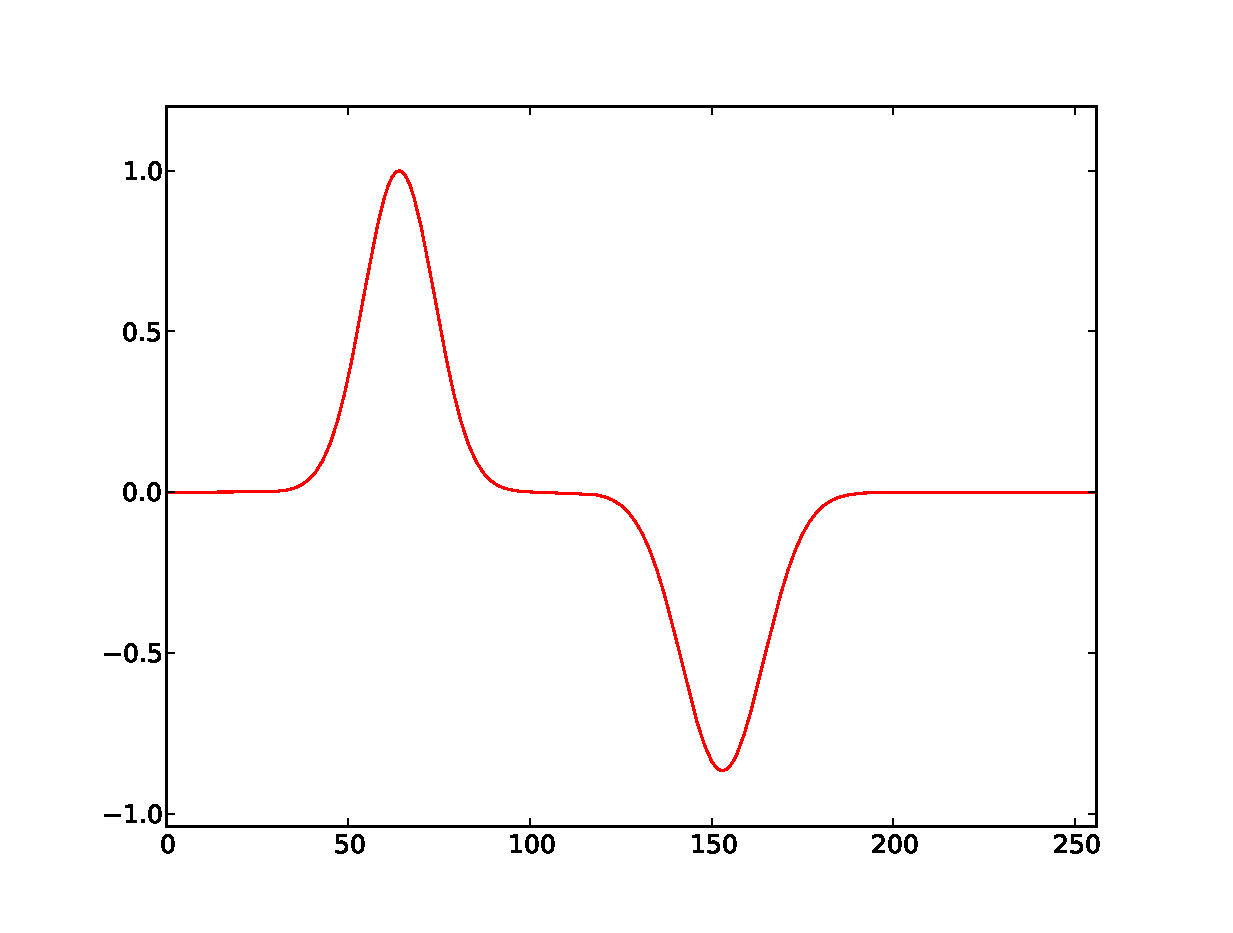
\includegraphics[width=3in,trim = 0 0 0 50]{./figures/signalSmooth.eps} &
%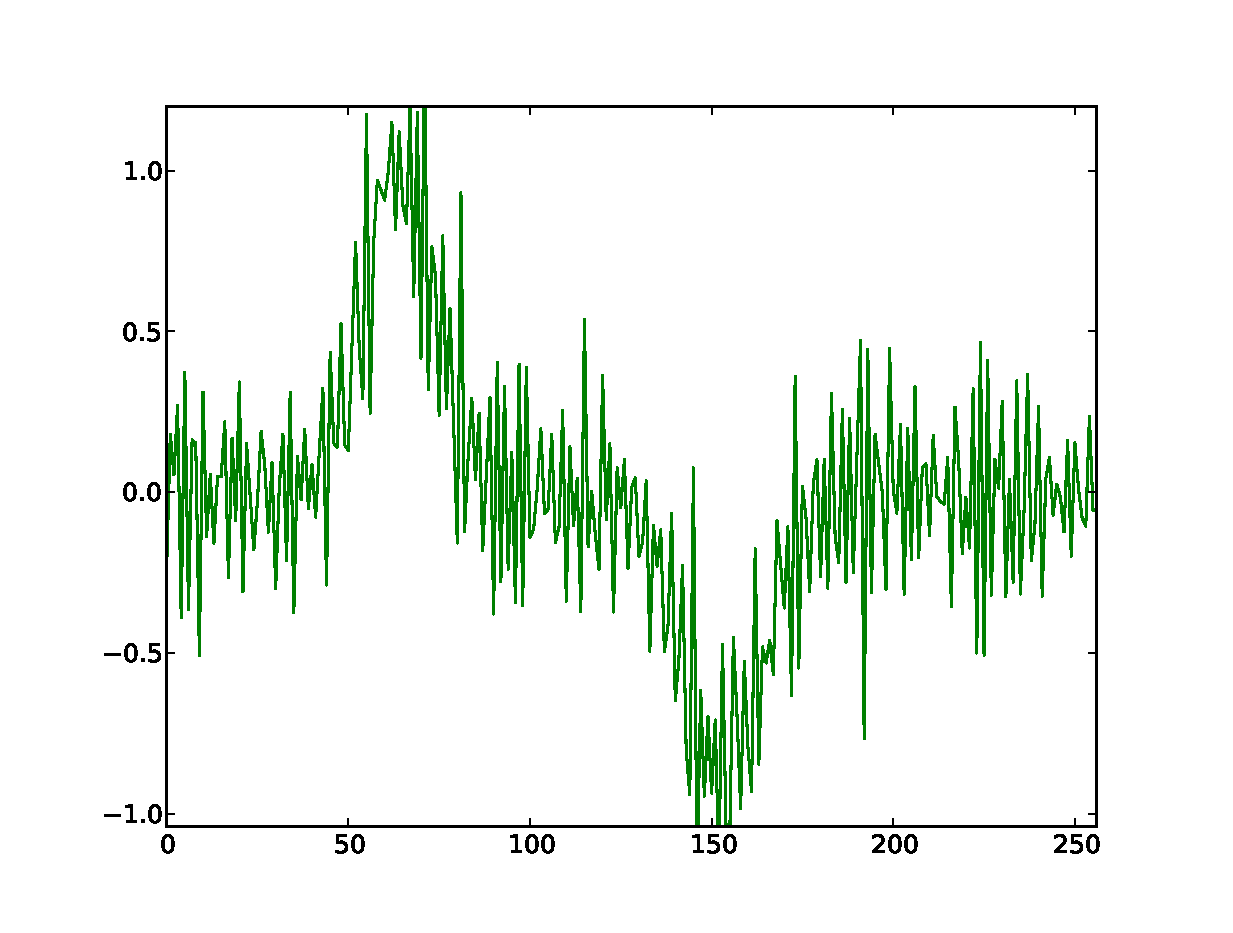
\includegraphics[width=3in,trim = 0 0 0 50]{./figures/Bn.eps} 
%\end{tabular}
%\end{table}
\end{block}
\begin{block}{Our Estimator:}
Chosen estimator is:
\begin{equation}
\hat\beta_{nj} = \left( 1 - \frac{\Omega_n^2 \epsilon^2}{\Delta_{nj} |B_{nj}|^2} \right)_+
\label{eq:betaEstimator}
\end{equation}
for $\Omega_n^2 := (p-2)\left(1 + \frac{\max_j \Delta_{nj}}{\min_j \Delta_{nj}}\right)$ . \\

An estimator of $\theta$ is formed via $\hat\theta_n = \Psi \hat \beta_n$.
\end{block}
            \begin{block}{Definitions:}
              Let the risk be:
              \[
              R(\hat\theta) = \mathbb{E}||\hat \theta - \theta ||_2^2
              \]
              and  define 
              \[
              \mathcal{E} := \{ \hat \theta = \Psi \lambda (B_n) : \lambda \in \mathbb{C}^p\}.
              \]
            \end{block}
          % 
          \vfill
          % 
        }
      \end{minipage}
    \end{beamercolorbox}
  \end{column}
%  % 
%  % 
%  % Column 3
%  % 
%  % 
  \begin{column}{.32\textwidth}
      \begin{beamercolorbox}[center,wd=\textwidth]{postercolumn}
        \begin{minipage}[T]{.95\textwidth} % tweaks the width, makes a new \textwidth
          \parbox[t][\columnheight]{\textwidth}{ % must be some better way to set 
%              %the the height, width and textwidth simultaneously
%              % Since all columns are the same length, it is all nice and tidy.  
%              % You have to get the height empirically
%              % ---------------------------------------------------------%
%              % fill each column with conten
            \begin{block}{Uniformly Consistent:}
              {\it  Let $\hat \beta_n$ be defined as in equation \eqref{eq:betaEstimator} and $\hat\theta_n = \Psi \hat\beta_n$.
                Then:}
              \begin{equation*}
                \limsup_{n \rightarrow \infty} \sup_{\theta \in \Theta} \, \gamma_n
                R\left(\hat \theta_n,\theta \right) < C < \infty
              \end{equation*}
              where  $\displaystyle{\gamma_n = \max_j \Delta_{nj}}$.
              %\small\textcolor{blue!75!white}{\textsc{ (Homrighausen and Genovese, 2011)}} 
            \end{block}
            \begin{block}{Satisfies an Oracle Inequality:}
              \normalsize
                  {\it Let
                    \[
                    R(\theta_*,\theta) = \argmin_{\hat \theta \in \mathcal{E}} R(\hat \theta,\theta)
                    \] 
                    be the risk of the $\mathcal{E}$ oracle.  Then
                    \begin{equation*}
                      R\left(\hat \theta_n,\theta \right) \leq R(\theta_*,\theta)(1 + O(1))
                    \end{equation*}
                    for a term $O(1)$ that does not depend on $\theta$.}
                  %\small \textcolor{blue!75!white}{\textsc{(Homrighausen and Genovese, 2011)}} 
            \end{block}

            \begin{block}{Simulations:}
              \begin{table}
                \centering
                \begin{tabular}{cccc}
                  $\theta_1$ and $K_i\theta_1$ & $\theta_2$ and $K_i\theta_2$
                  & \multicolumn{2}{c}{Examples of Observations} \\
                  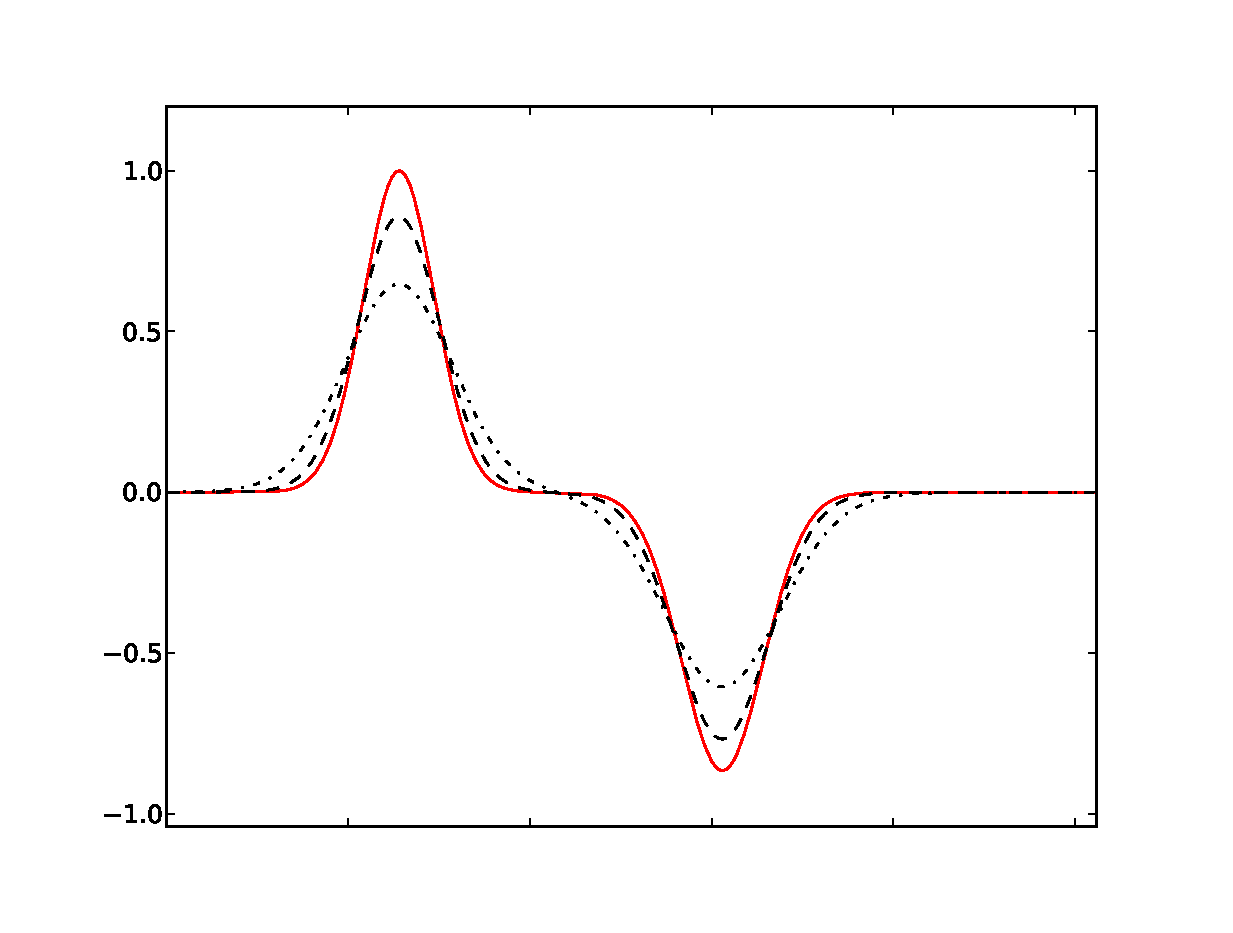
\includegraphics[width=3.4in,trim=0 30 0 0,clip]{./figures/thetasmooth.eps} &
                  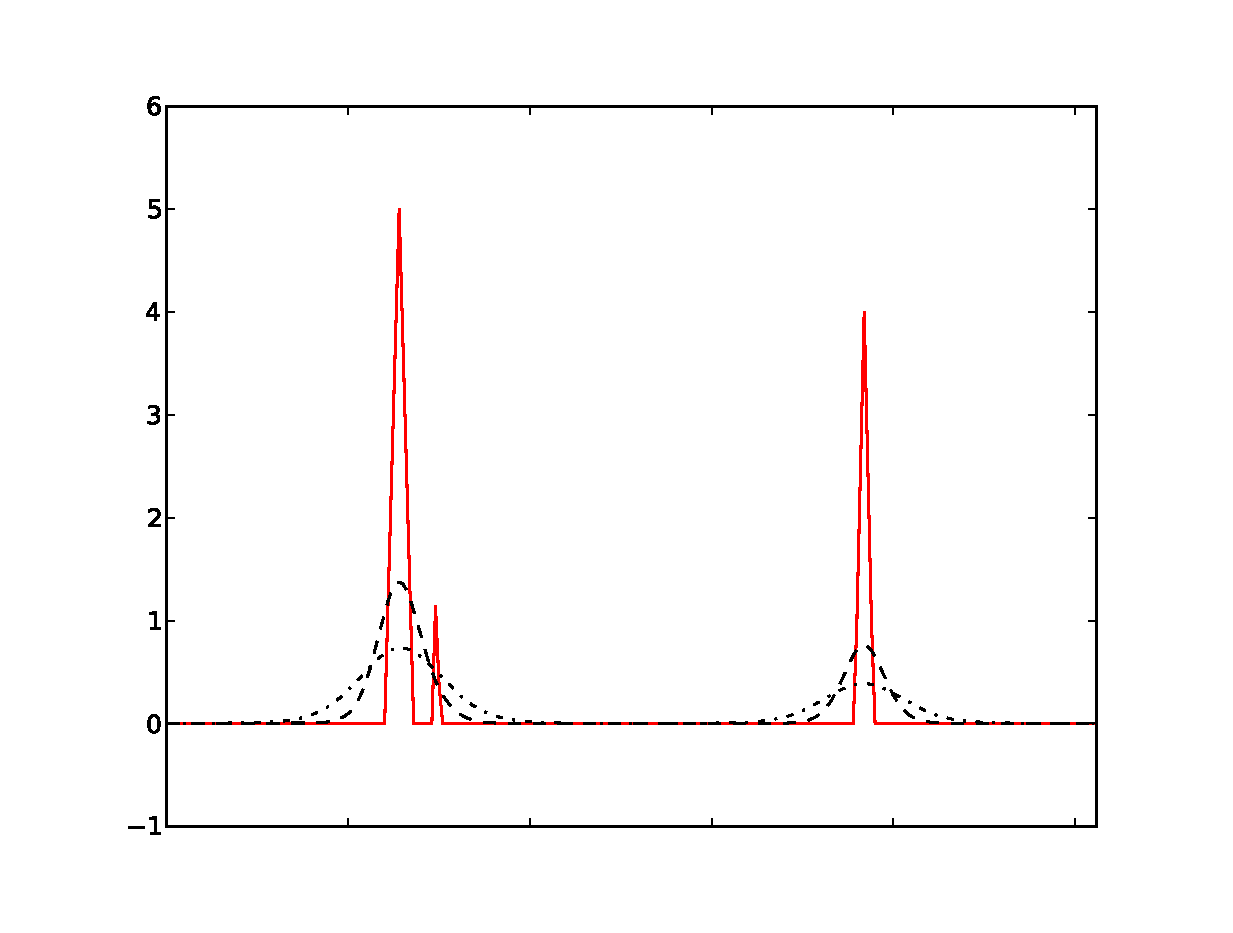
\includegraphics[width=3.4in,trim=0 30 0 0,clip]{./figures/thetapeaked.eps} &
                  \includegraphics[width=3.4in,trim=0 30 0 0,clip]{./figures/thetasmoothDataPlot0.eps} &
                  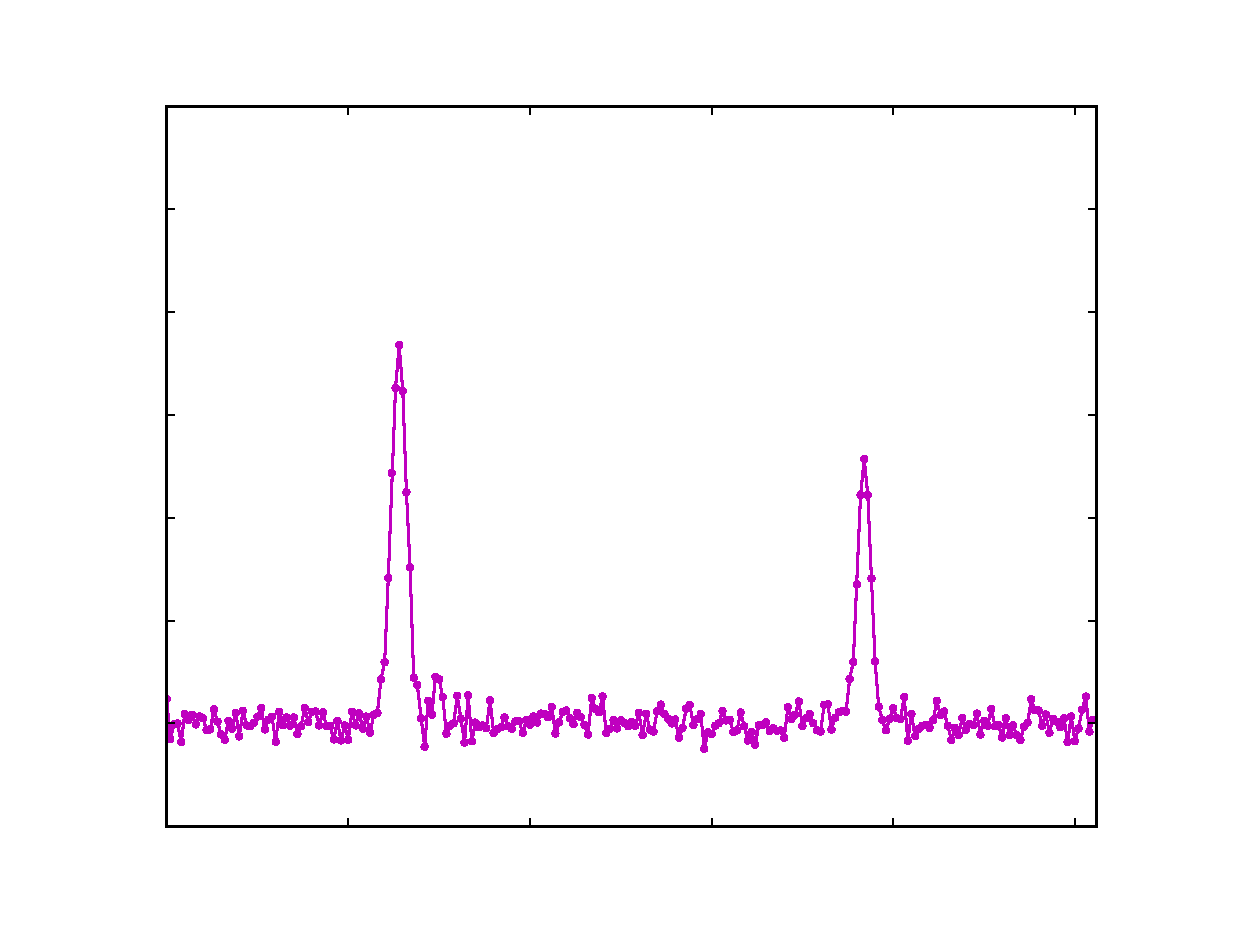
\includegraphics[width=3.4in,trim=0 30 0 0,clip]{./figures/thetapeakedDataPlot2.eps} \\
                \end{tabular}
              \end{table}
            \end{block}
            \begin{block}{Reconstructions:}
              \begin{table}
                \centering
                \begin{tabular}{cccc}
                  $\hat\theta_n$ & $\hat \theta_{\text{GCV}}$ & $\hat\theta_n$ & $\hat \theta_{\text{GCV}}$ \\
                  \multicolumn{4}{l}{$n = 50$}  \\
                  \includegraphics[width=3.4in,trim=0 30 0 0,clip]{./figures/minesmooth200.eps} &
                  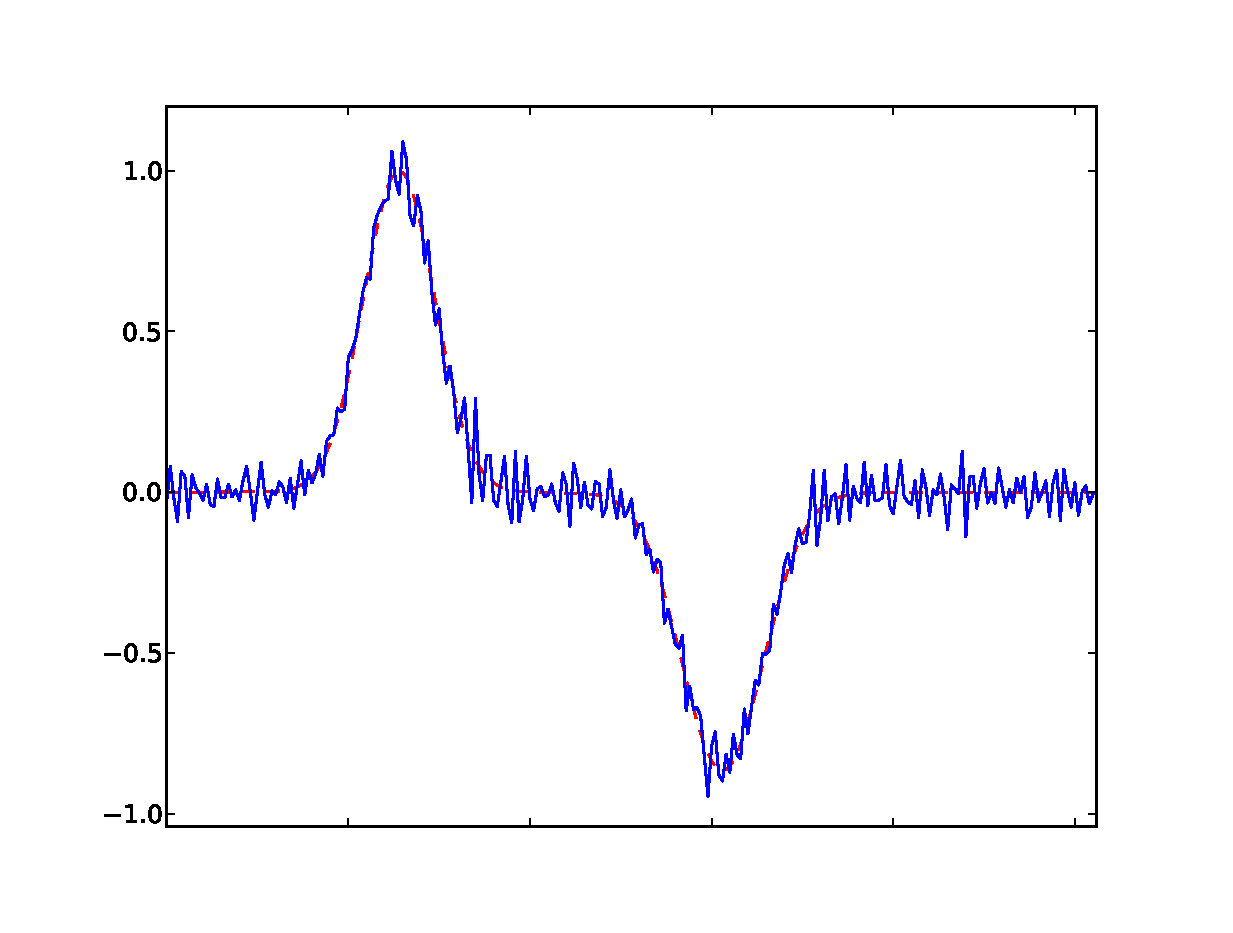
\includegraphics[width=3.4in,trim=0 30 0 0,clip]{./figures/GCVsmooth100.eps} &
                  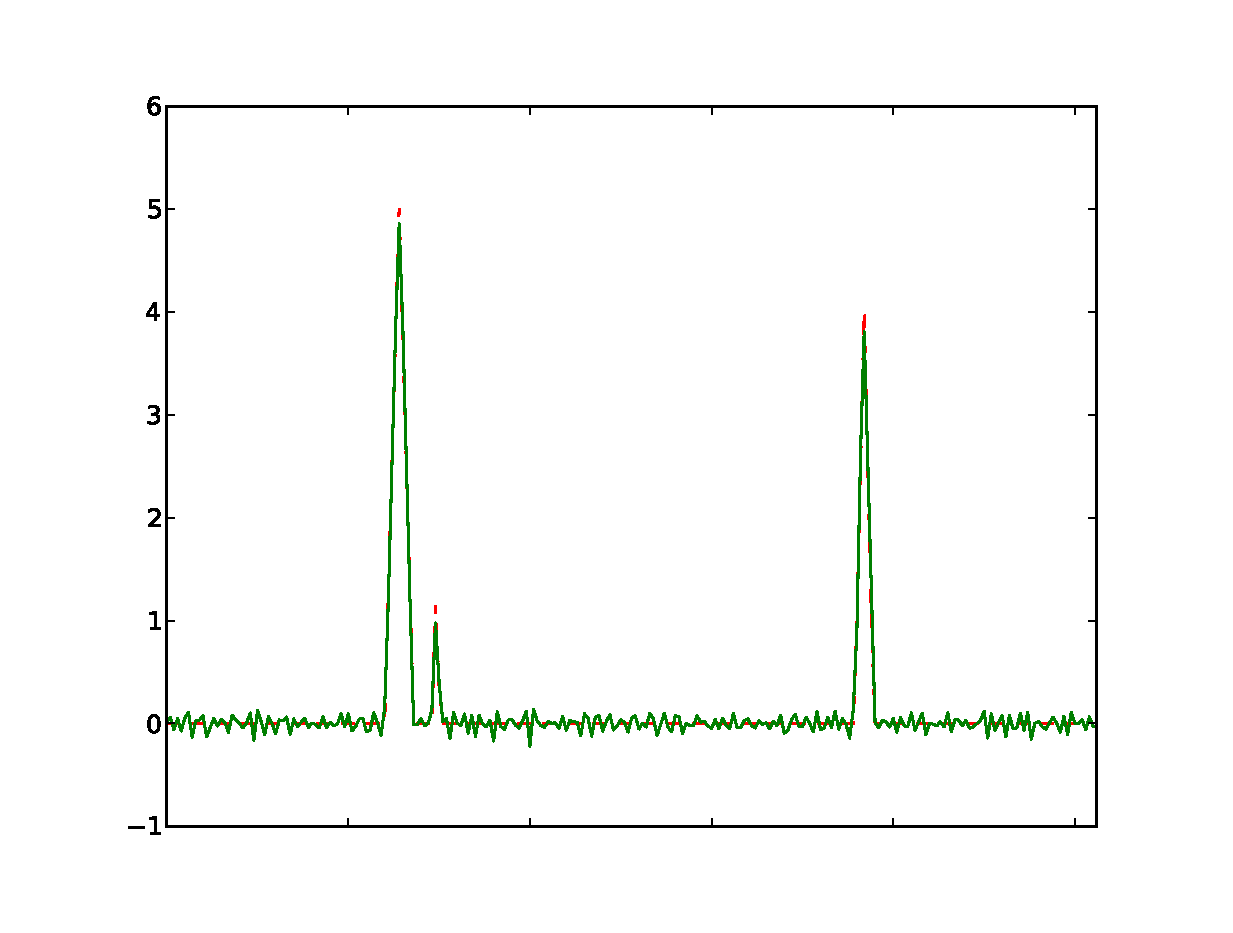
\includegraphics[width=3.4in,trim=0 30 0 0,clip]{./figures/minepeaked100.eps} &
                  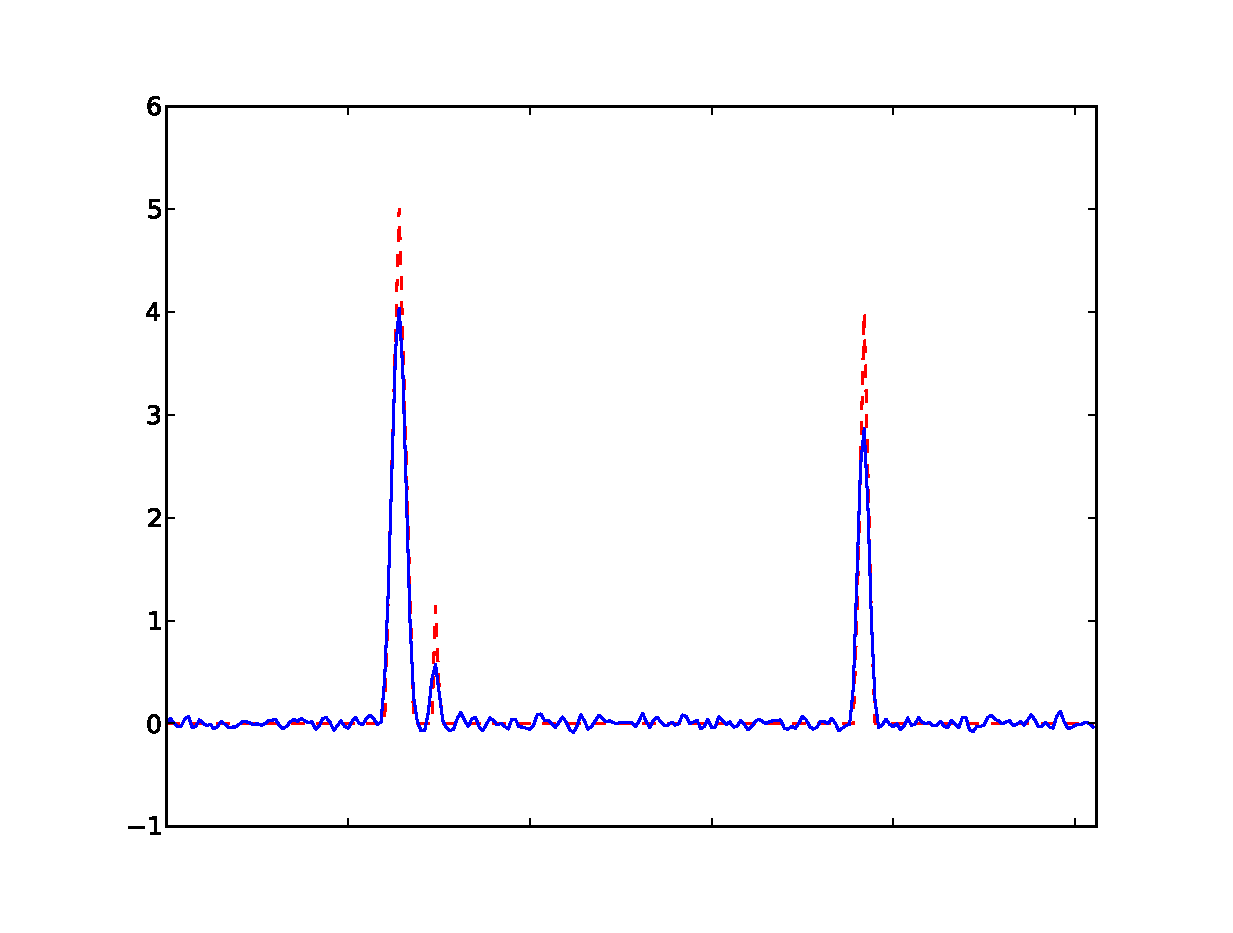
\includegraphics[width=3.4in,trim=0 30 0 0,clip]{./figures/GCVpeaked15.eps} \\
                  \multicolumn{4}{l}{$n = 100$}  \\
                  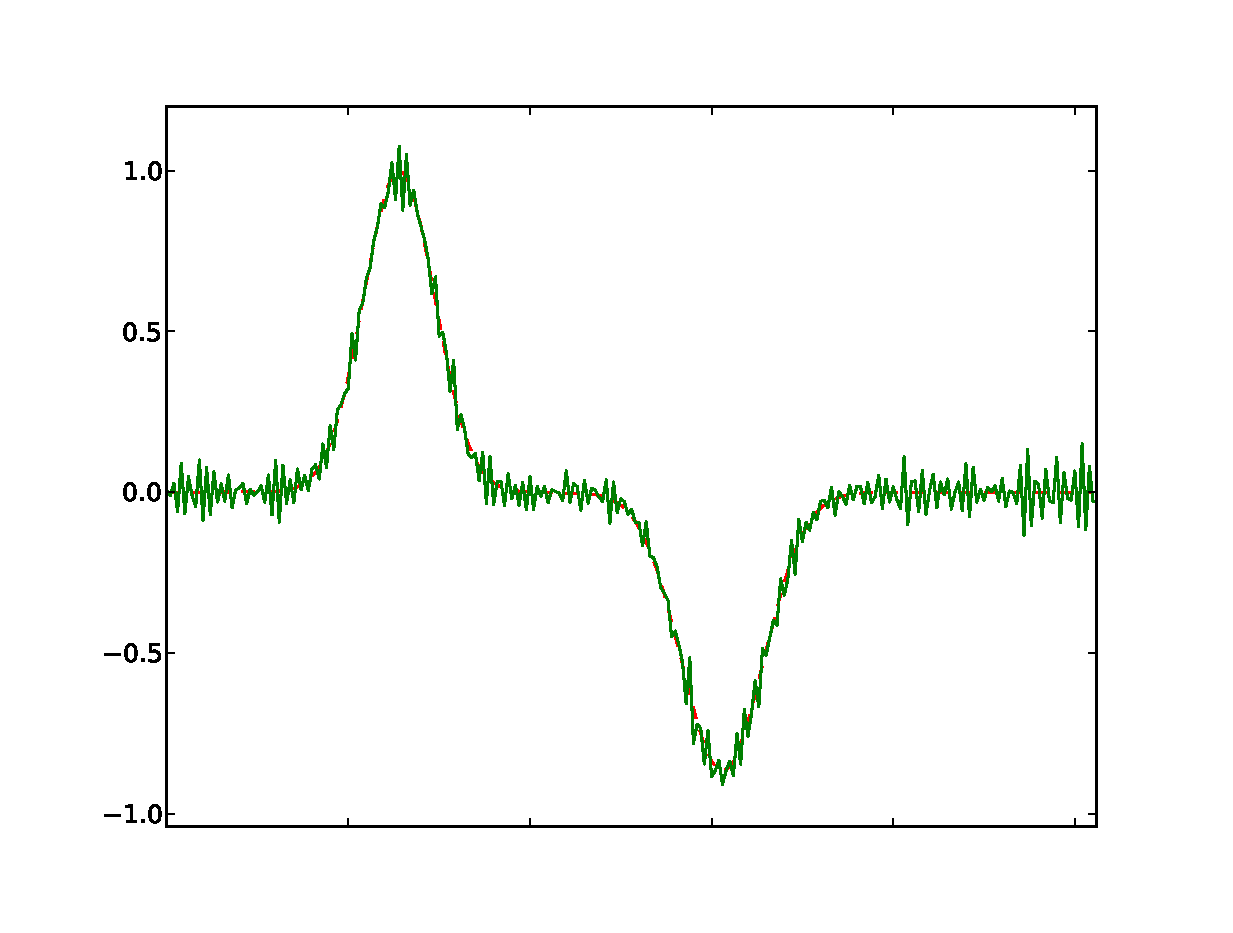
\includegraphics[width=3.4in,trim=0 30 0 0,clip]{./figures/minesmooth300.eps} &
                  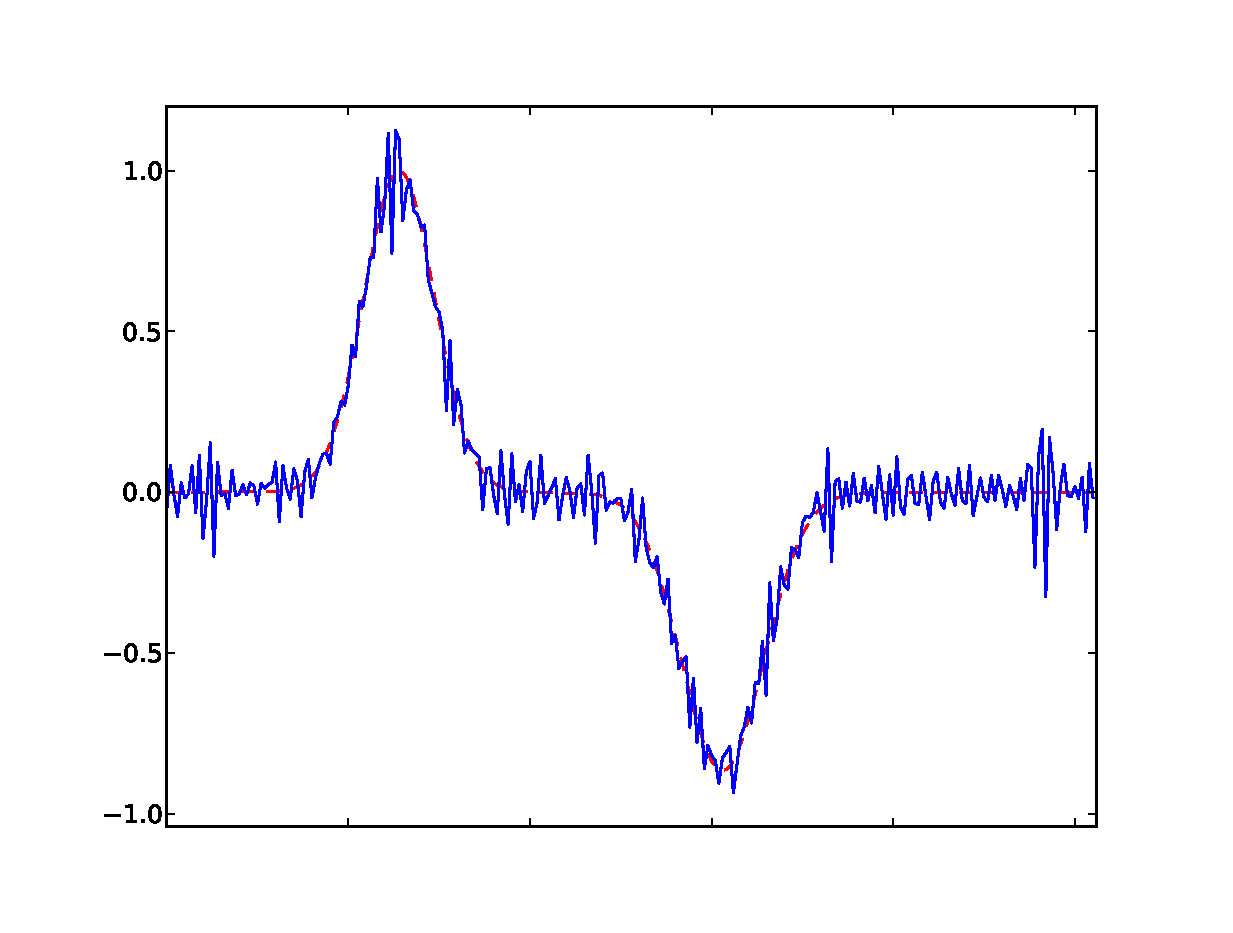
\includegraphics[width=3.4in,trim=0 30 0 0,clip]{./figures/GCVsmooth200.eps} &
                  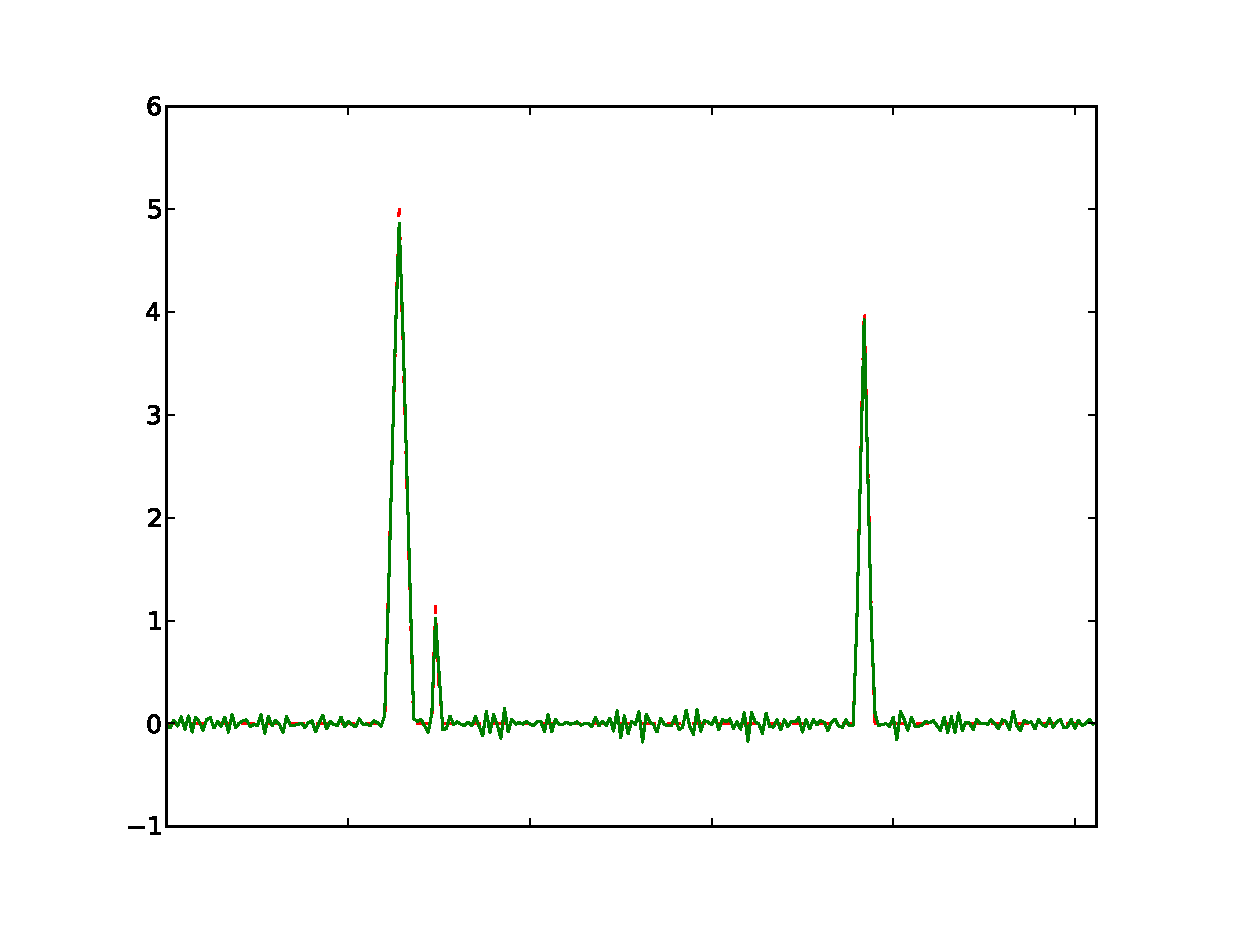
\includegraphics[width=3.4in,trim=0 30 0 0,clip]{./figures/minepeaked200.eps} &
                  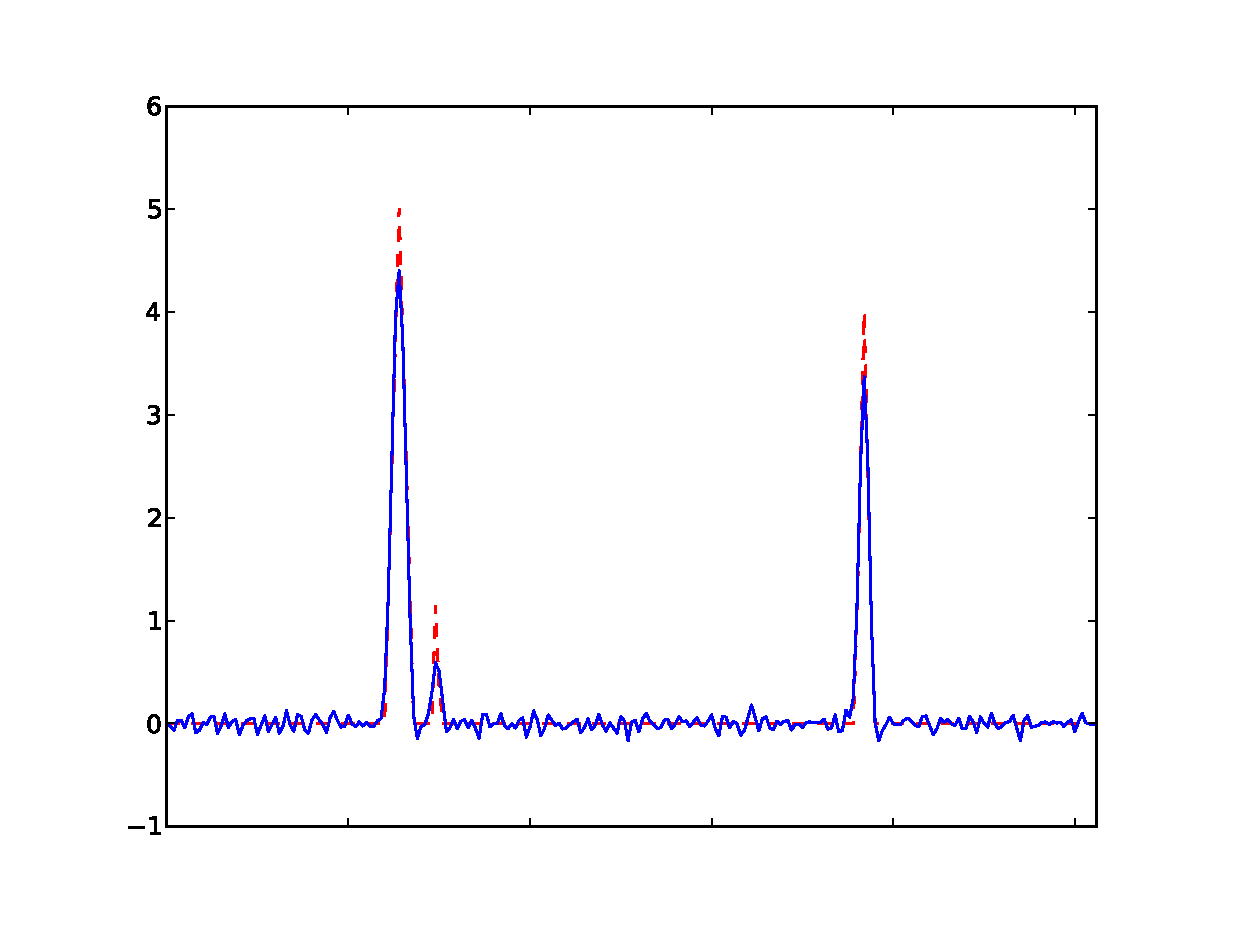
\includegraphics[width=3.4in,trim=0 30 0 0,clip]{./figures/GCVpeaked30.eps} \\
%                  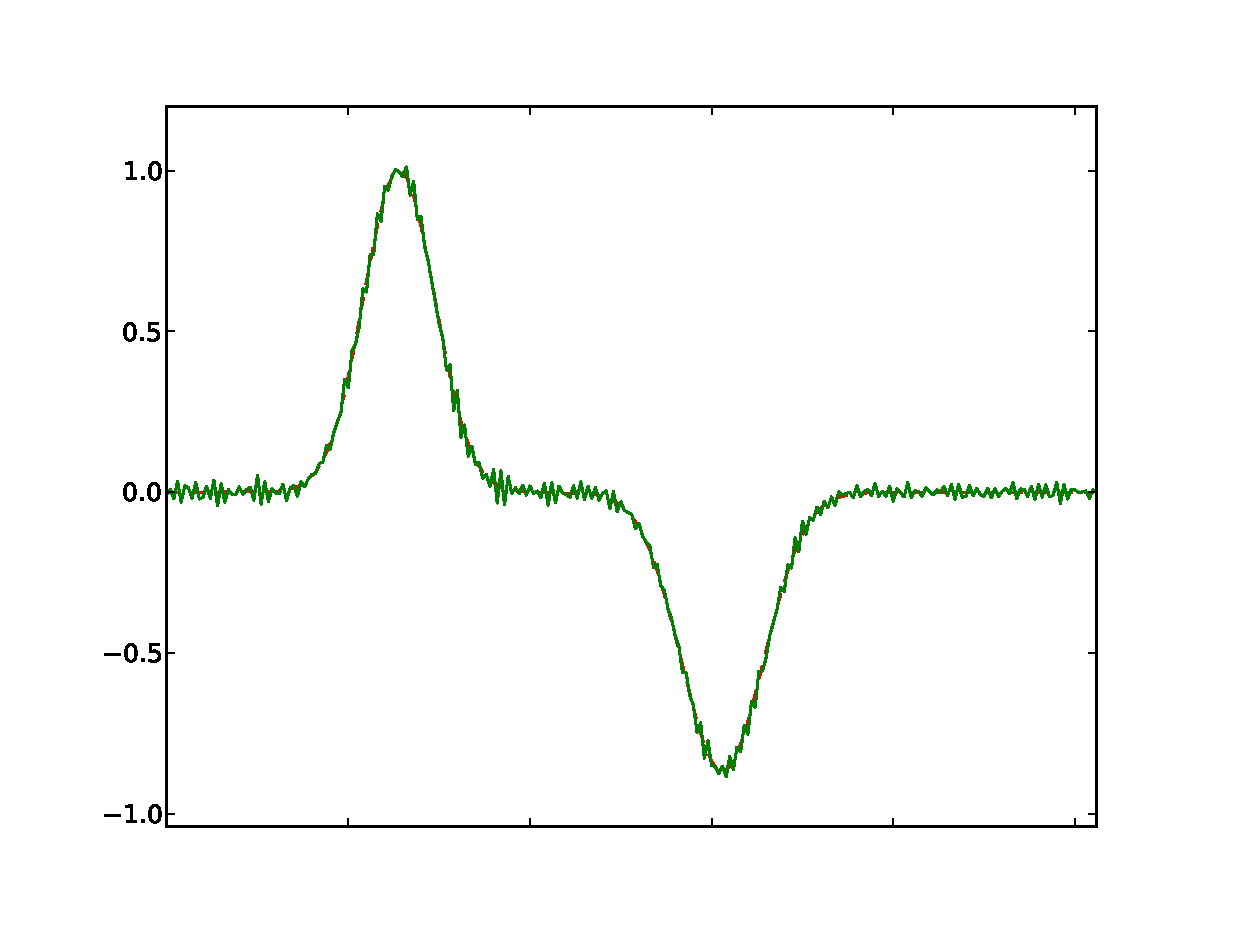
\includegraphics[width=3.5in,trim=0 30 0 0,clip]{./figures/minesmooth800.eps} &
%                  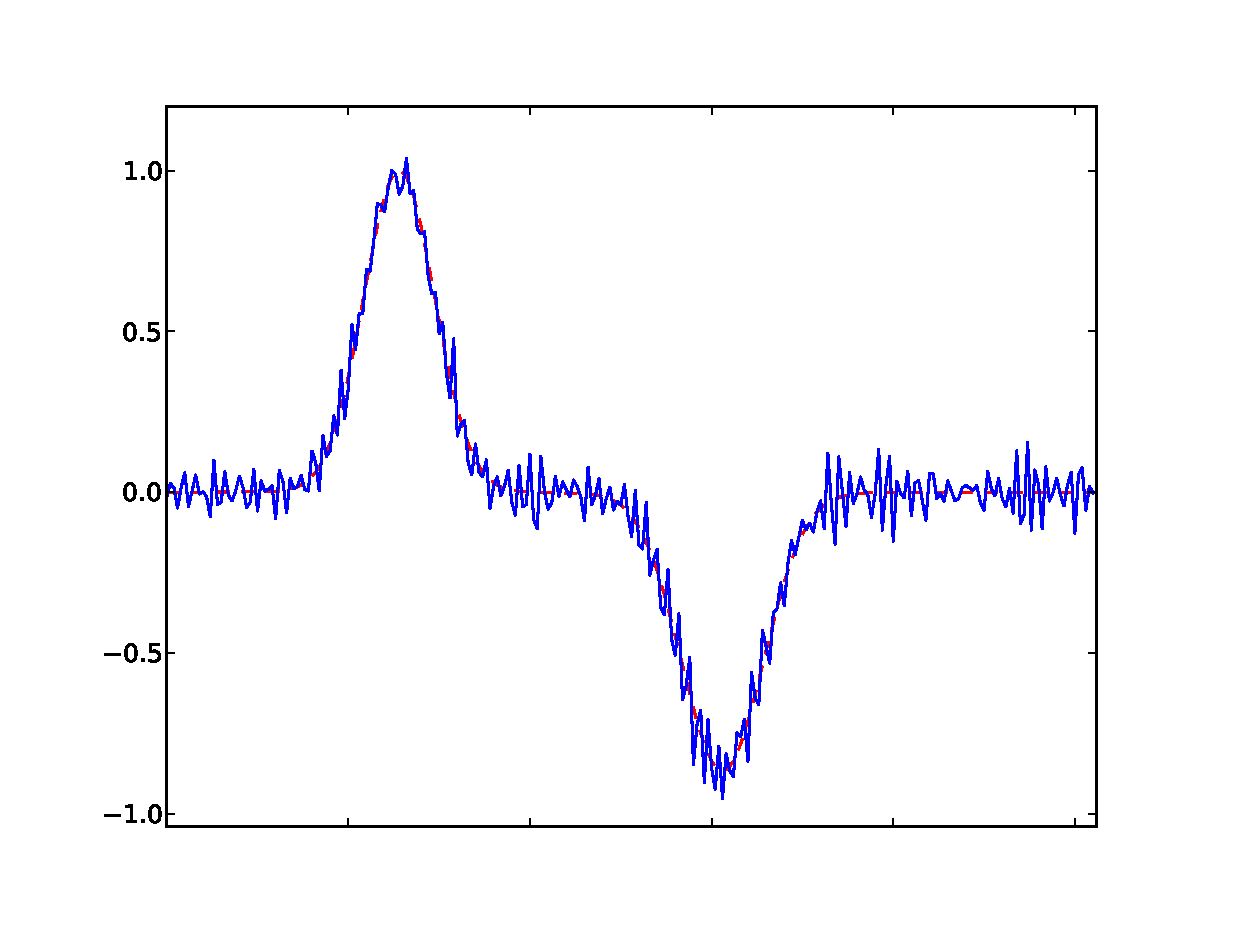
\includegraphics[width=3.5in,trim=0 30 0 0,clip]{./figures/GCVsmooth300.eps} &
%                  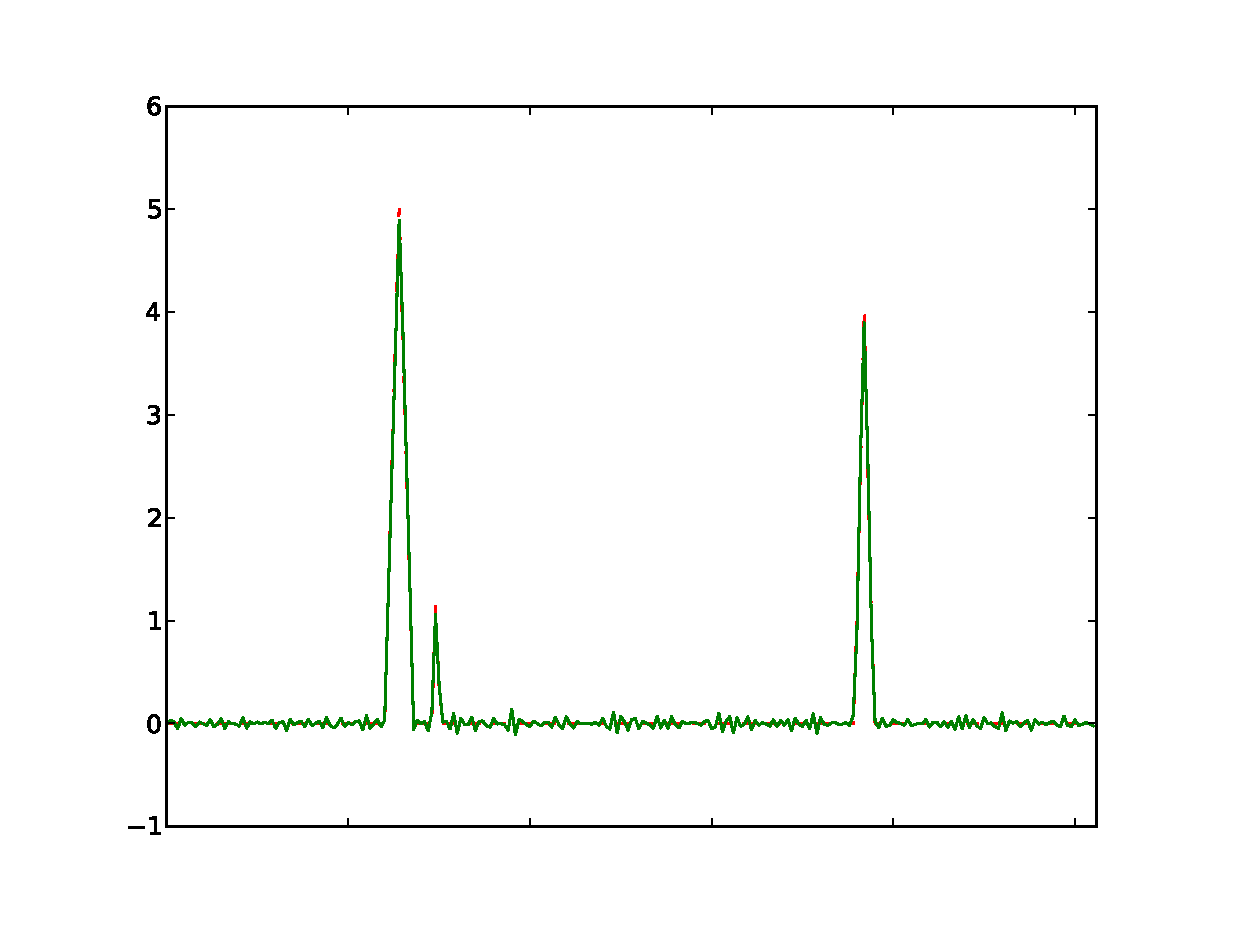
\includegraphics[width=3.5in,trim=0 30 0 0,clip]{./figures/minepeaked500.eps} &
%                  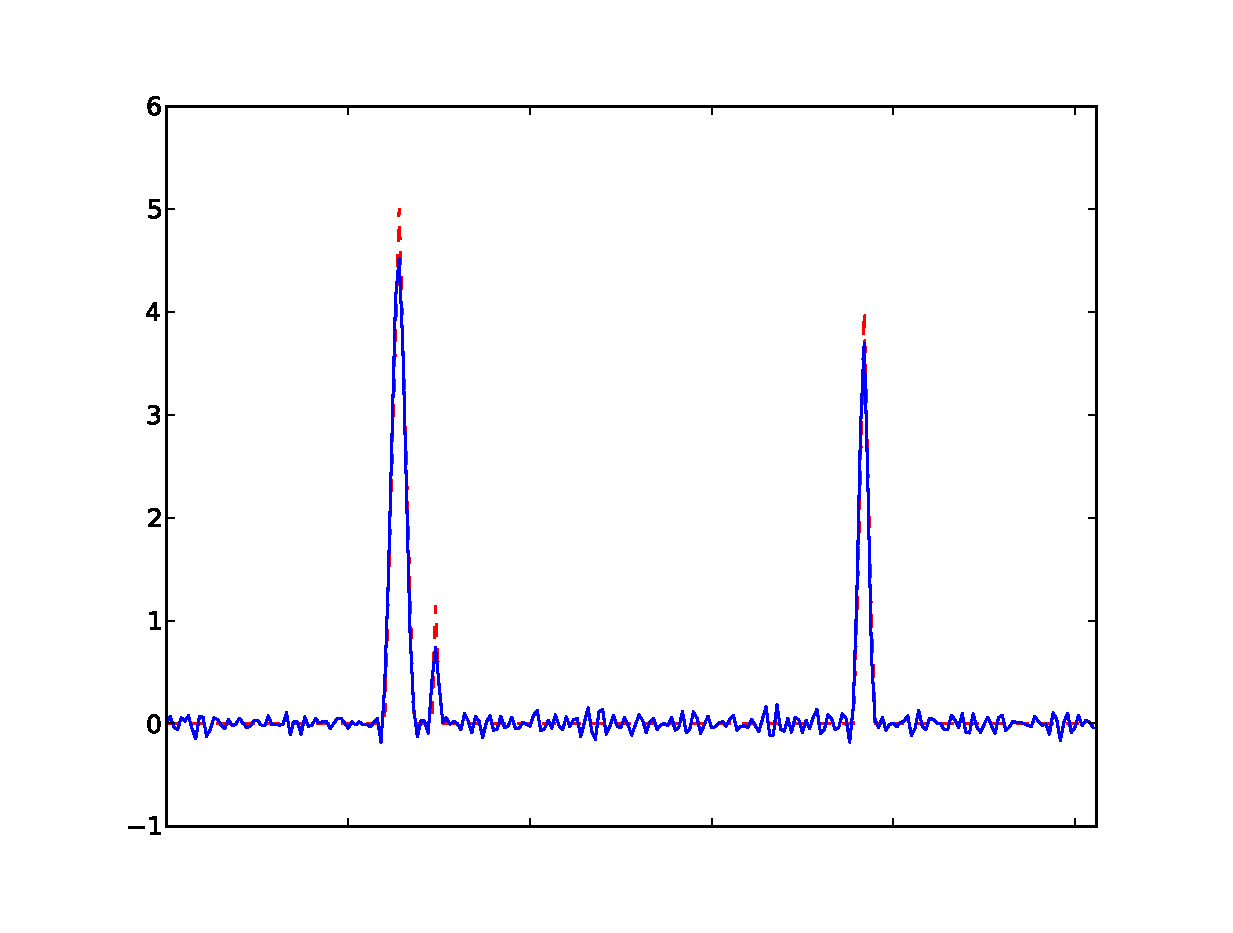
\includegraphics[width=3.5in,trim=0 30 0 0,clip]{./figures/GCVpeaked50.eps} \\       
                  \multicolumn{4}{l}{$n = 200$}  \\
                  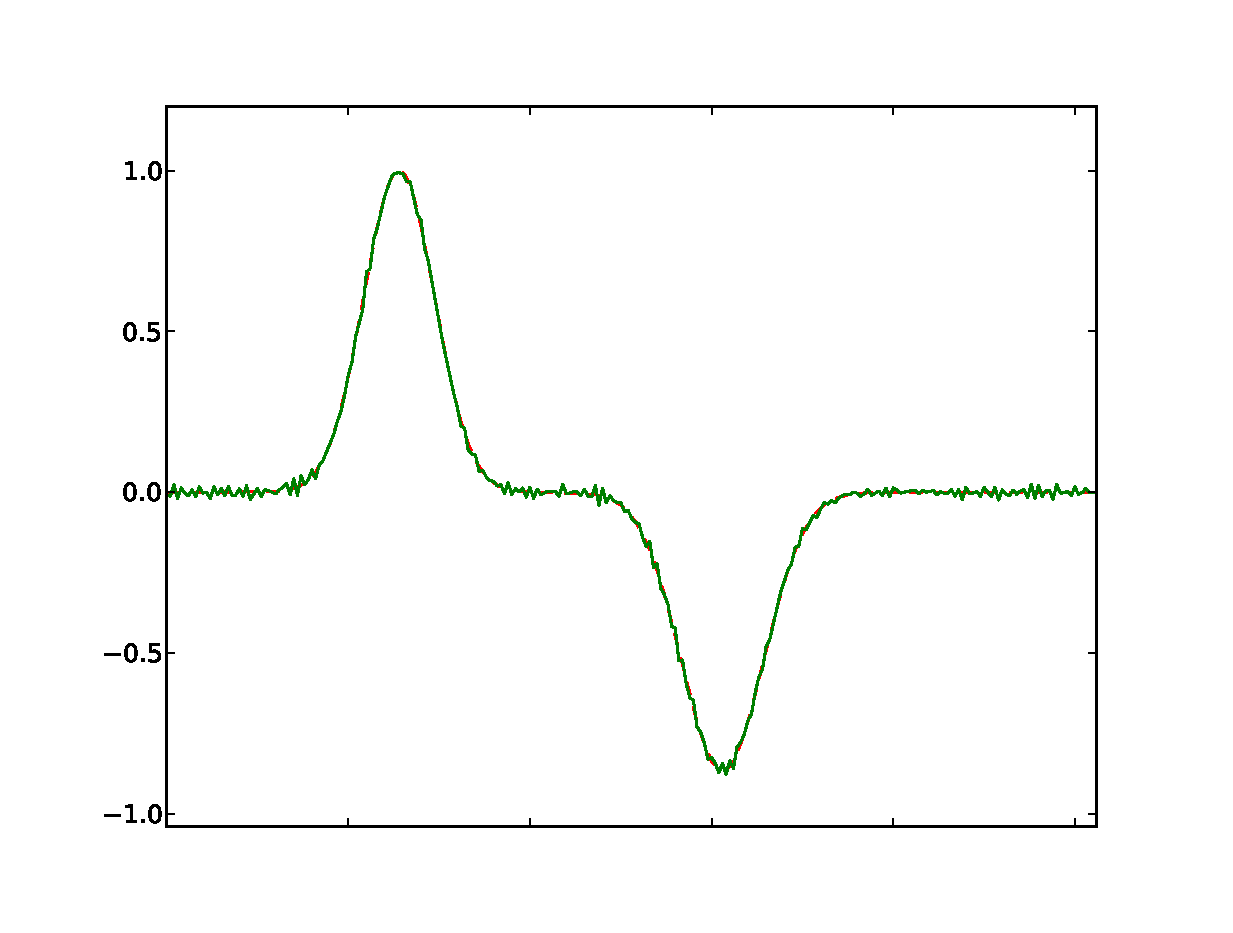
\includegraphics[width=3.4in,trim=0 30 0 0,clip]{./figures/minesmooth1500.eps} &
                  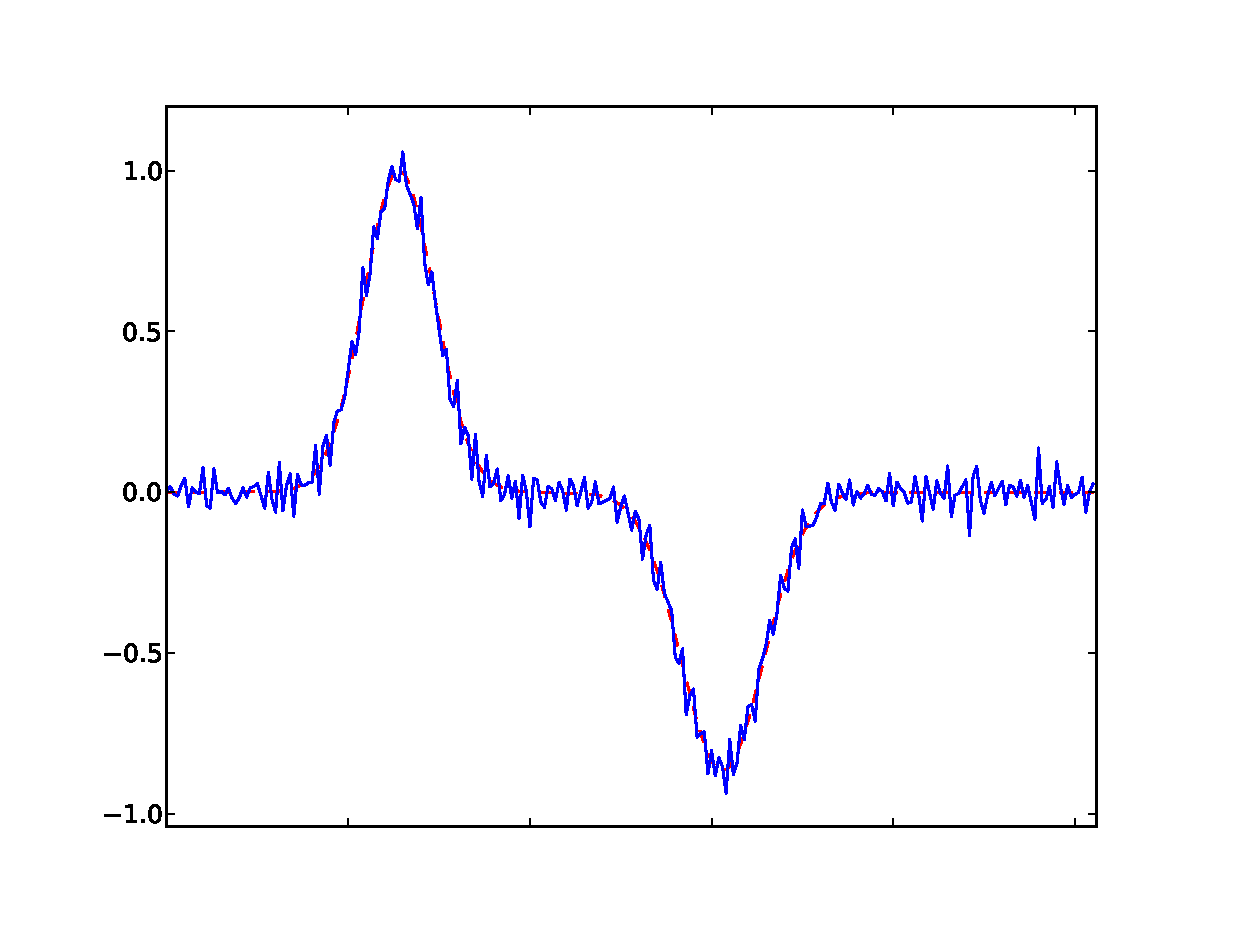
\includegraphics[width=3.4in,trim=0 30 0 0,clip]{./figures/GCVsmooth500.eps} & 
                  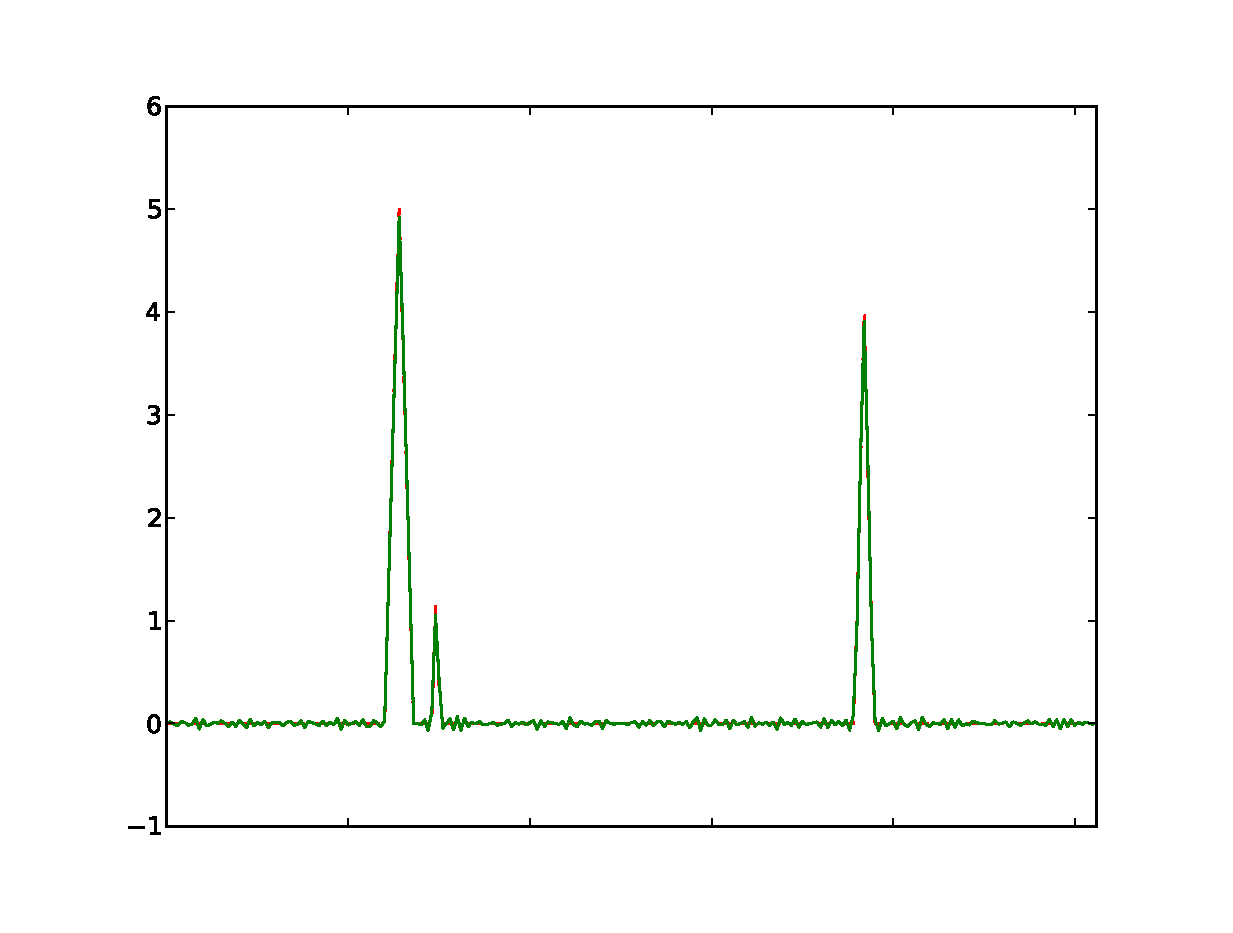
\includegraphics[width=3.4in,trim=0 30 0 0,clip]{./figures/minepeaked1000.eps}&
                  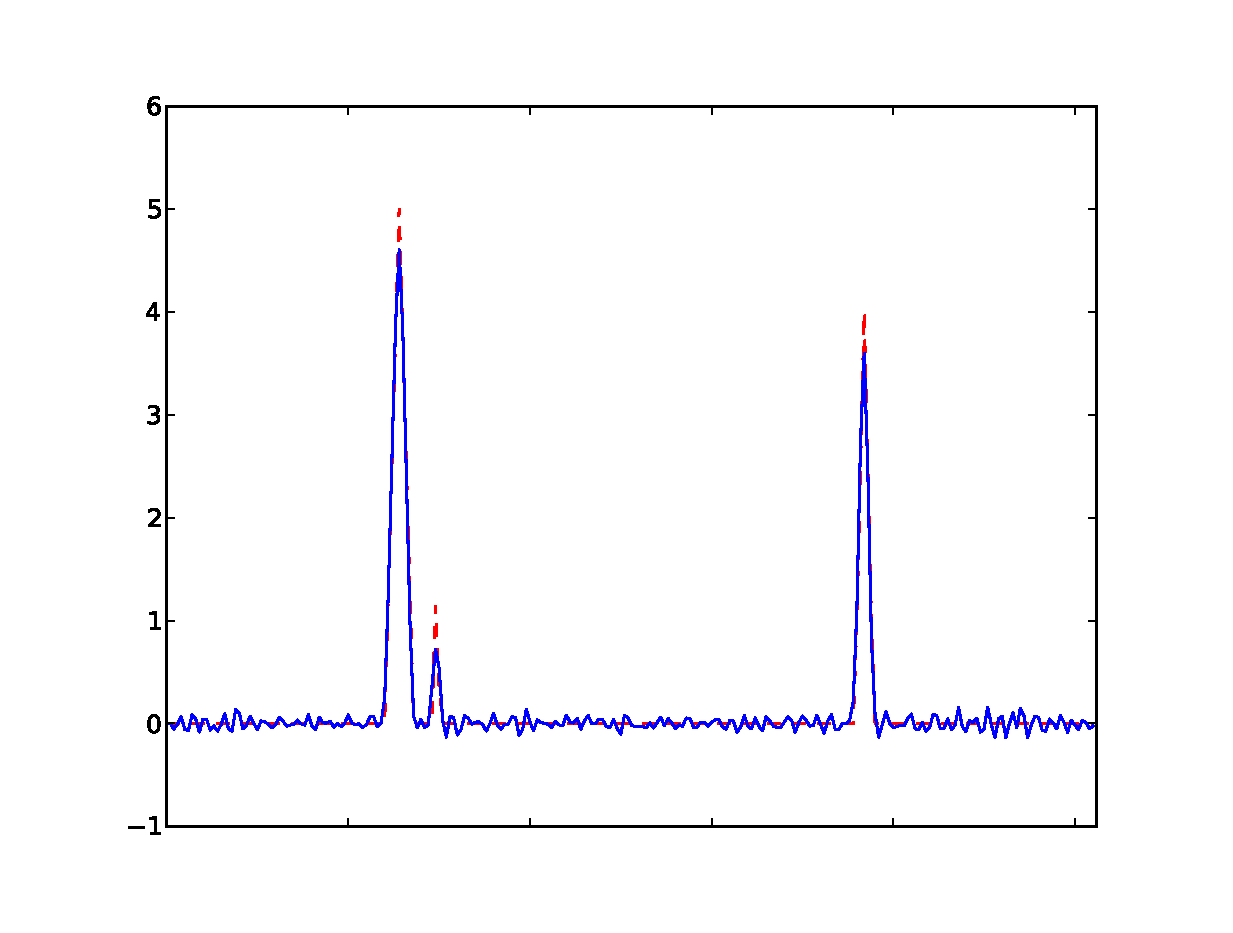
\includegraphics[width=3.4in,trim=0 30 0 0,clip]{./figures/GCVpeaked40.eps} 
                \end{tabular}
              \end{table}

              \begin{table}[!h]
                \begin{tabular}{l|cc|cc}
                  & $RR(\hat\theta_n,\theta_1)$ & $RR(\hat\theta_{\text{GCV}},\theta_1)$
                  & $RR(\hat\theta_n,\theta_2)$ & $RR(\hat\theta_{\text{GCV}},\theta_2)$ \\
                  \hline
                  $n = 50$             & 0.210              & 0.223       & 0.116              & 0.171 \\
                  $n = 100$             & 0.149              & 0.199       & 0.092              & 0.149 \\
                  $n = 200$             & 0.120              & 0.173       & 0.079              & 0.141   
                \end{tabular} 
              \end{table}
              \[
              RR(\hat\theta,\theta) = \sqrt{\frac{R(\hat \theta,\theta)}{||\theta||^2}}
              \]
            \end{block}
          % 
          \vfill
          % 
          }
        \end{minipage}
      \end{beamercolorbox}
    \end{column}
  \end{columns}
\end{frame}
\end{document}

